\documentclass[11pt, a4paper, openany, oneside, dvipdfmx]{jsbook}
\let\cleardoublepage\clearpage
%\documentclass[a4paper,uplatex,dvipdfmx,ja=standard,12pt,jafont=noalphabet,openany,oneside,draft]{bxjsbook} % draft
\usepackage{amsthm, amsfonts, amsmath}
\usepackage[print]{Thesis}
%\usepackage[phd]{Thesis}
\usepackage{color}
\usepackage{graphicx}
\usepackage{listings,jvlisting}
\usepackage{here, latexsym, bm, ascmac, mathtools, multicol, tcolorbox, graphicx, comment, pgfplots}
\usepackage{algpseudocode}
\usepackage{algorithm}
\usepackage{tikz}
\usepackage{siunitx}
\usepackage{subcaption}
\usepackage{booktabs}
\usepackage{pxjahyper}
\usepackage{xcolor}



\usetikzlibrary{intersections}

\usepgfplotslibrary{fillbetween}


\hypersetup{
    colorlinks=true,
    citecolor=blue,
    linkcolor=blue,
    urlcolor=orange,
}


\newtheorem{thm}{Theorem}[section]
\newtheorem{cor}{Corollary} [section]
\newtheorem{lem}{Lemma}[section]
\newtheorem{prop}{Proposition}[section]
\theoremstyle{definition}
\newtheorem{dfn}{Definition}[section]
\newtheorem{ex}{Example}[section]
\newtheorem{rem}{Remark}[section]
\newtheorem{ass}{Assumption}[section]
\newtheorem*{monge}{Mongeの最適輸送問題}
\newtheorem*{Kantorovich}{Kantorovich双対問題}

\renewcommand{\labelenumii}{(\roman{enumii})}
\renewcommand{\labelenumi}{(\arabic{enumi})}

%%%%%%%%% タイトルページの設定 %%%%%%%%%%%%%%%%%%

\nendo{5}
\thesistype{修士}
\title{最適輸送法を用いた偏微分方程式のソルバー}
\etitle{PDE solver using optimal transport}
\kyokanA{}{POZAR NORBERT 准教授}
\affiliation{金沢大学大学院 自然科学研究科}
\major{博士前期課程 数物科学専攻}

\regnum{2215011016}
\author{坂井幸人}
%%%%%%%%%%%%%%%%%%%%%%%%%%%%%%%%%%%%%%%%%%%%%


\begin{document}
\maketitle
% \makeatletter\@openrightfalse\makeatother
\frontmatter
\tableofcontents
% \listoffigures
% \listoftables

\mainmatter
\chapter{イントロダクション} \label{ch:intro}

近年、最適輸送問題(Optimal Transport Problem, OTP)と偏微分方程式の間に深い関係が発見されたことから最適輸送問題への関心が高まっている。
偏微分方程式 を解くための新しい方法として、最適輸送問題の解法を用いるソルバーが注目されている。
そんな中発表されたJacobsとLégerによって導入された the back-and-forth method は、最適輸送問題のソルバーを用いた偏微分方程式の新たな解法が発表された\cite{MR4238775}。
この解法は特に非線形偏微分方程式に有効であり、今までの解法に比べて高速でかつ安定性条件を必要としないため、より幅広い問題を解くことが可能である。
私はこの最適輸送問題を用いた偏微分方程式のソルバーに興味がある。

本研究では、特に以下の偏微分方程式について考える。
\begin{align}
    \begin{split}
        \label{eq:Darcy's}
        \partial_t \rho - \nabla \cdot (\rho \nabla \varphi) = 0, \\
        \varphi = \delta U(\rho).
    \end{split}
\end{align}
この偏微分方程式(\ref{eq:Darcy's})は、以下のエネルギー関数$U$用いることで多孔質媒体方程式(Porous medium equation, PME)となる。
$$
    U(\rho) = \frac{\gamma}{m - 1} \int \rho^m \,dx \quad(m > 1, \gamma > 0)
$$
ここで、多孔質媒体方程式 は、多孔質媒体中での流体流動を記述する以下の偏微分方程式である。
\begin{align}
    \begin{split}
        \label{eq:PME}
        \partial_t \rho - \gamma\Delta(\rho^m) = 0  \quad(m > 1, \gamma > 0)
    \end{split}
\end{align}

一般的に多孔質媒体方程式 は、剛性があり非線形であり、数値的に解くのは困難である。
そのため本研究では、偏微分方程式のJacobs、Lee、Légerによって導入された the back-and-forth methodを用いたソルバーと他のソルバーとの比較を行い、
特定の条件下においてback-and-forth methodのソルバーが、非線形な多孔質媒体方程式をより効率的に解くことができることを示す。


\begin{comment}
研究では、以下の研究内容を検討します。

* BFM を PME に適用するための一般化
* 提案するソルバーの効率性の評価
* 提案するソルバーの他のソルバーとの比較

BFM を PME に適用するためには、以下の点に留意する必要があります。

* PME は、剛性があり非線形な方程式であるため、BFM の解法の適応が必要となる。
* PME の境界条件は、通常、PDE の解法に固有の形状となる。BFM の解法では、これらの境界条件をどのように扱うかが課題となる。

提案するソルバーの効率性を評価するためには、以下の点に留意する必要があります。

* ソルバーの収束精度と収束速度を評価する。
* ソルバーの計算コストを評価する。

提案するソルバーと他のソルバーとの比較を行うためには、以下の点に留意する必要があります。

* ソルバーの収束精度と収束速度を比較する。
* ソルバーの計算コストを比較する。

本研究では、これらの点に留意して、提案するソルバーの有効性を検証します。

\end{comment}
















\section{全体のアプローチ}
\label{sect:全体のアプローチ}
本論文では、$\Omega$を凸であり、コンパクトな$\mathbb{R}^n$の部分集合と仮定する。
また次の条件に従うものとする。
\begin{dfn}
\label{dfn:1}
    $\Omega$ 上の確率測度であり、非負の測度で質量(mass)が1である確率測度の集合を $\mathcal{P} (\Omega)$ とする。
    また、$\Omega$上の連続関数の空間を$C(\Omega)$で表す。
    簡単のために積分が \(1\) となる非負の \(L^1(\mathbb{R}^n)\)関数 で考える。
\end{dfn}

非線形の偏微分方程式である多孔質媒体方程式は、エネルギー関数$U$に基づくWasserstein 勾配流として表現できる。
これにより、時間離散化を行い変分原理に基づき以下の反復を行うことによって多孔質媒体方程式の近似解を求めるJKOスキームを行うことができる。
ただし、$\rho$は最小化問題(\ref{eq:minimizer})の解である。さらに、(\ref{eq:JKOscheme})を一般化最適輸送問題という。
\begin{equation}
    \label{eq:minimizer}
    \min_{\rho \in \mathcal{P}} U(\rho) + \frac{1}{2\tau} W_2^2(\rho, \mu)
\end{equation}
\begin{equation}
    \label{eq:JKOscheme}
    \rho^{(n+1)} := \underset{\rho}{\operatorname{argmin}}\, U(\rho) + \frac{1}{2\tau} W_2^2(\rho, \rho^{(n)})
\end{equation}
ここで、2-Wasserstein距離のKantorovichの双対公式は次のように表される:

\begin{equation}
    \label{eq:wasserstein dual}
    \frac{1}{2\tau} W_2^2(\rho, \mu) = \sup_{(\varphi, \psi) \in \mathcal{C}} \left( \int \varphi d\rho + \int \psi d\mu \right)
\end{equation}

ここで、$\mathcal{C}$は制約
\[
    \mathcal{C}  := \{(\varphi, \psi) \in C(\Omega) \times C(\Omega) : \varphi(x) + \psi(y) \leq \frac{1}{2 \tau} |x - y|^2 \}
\]
を満たす関数$(\varphi, \psi)$の集合、$\tau$はスキーム内の時間ステップを表す。
重要な点として、集合$\mathcal{C}$は凸であることに注意する。

双対形式を用いることで、
\begin{align*}
    \min_{\rho \in \mathcal{P}} U(\rho) + \frac{1}{2\tau} W_2^2(\rho, \mu) &= \min_{\rho \in \mathcal{P}} \left(U(\rho) + \sup_{(\varphi, \psi) \in \mathcal{C}} \left(\int \varphi \, d\rho + \int \psi \, d\mu\right)\right)\\
                                                                            &= \min_{\rho \in \mathcal{P}} \sup_{(\varphi, \psi) \in \mathcal{C}} \left(U(\rho) + \int \varphi \, d\rho + \int \psi \, d\mu\right)
  \end{align*}
  次に、\(\mathcal{P}\)と\(\mathcal{C}\)が凸であり、\(U\)が凸であるとすると、関数
  \[
    \label{eq:L}
    L(\rho, (\varphi, \psi)) := U(\rho) + \int \varphi \, d\rho + \int \psi \, d\mu
  \]
  は\hypertarget{rho_convex}{\(\rho\)に関して凸関数}(\((\varphi, \psi)\)が固定された場合)、
  および\hypertarget{varphipsi_concave}{\((\varphi, \psi)\)に関しては凹関数}になる。
  このため、\cite[Proposition 2.4 (p176)]{MR1727362}のような最小最大の定理を適用して、\(\min\)と\(\sup\)の順序を交換することができる。
  したがって、
  \begin{align}
    \label{eq:dual}
    \min_{\rho \in \mathcal{P}} U(\rho) + \frac{1}{2\tau} W_2^2(\rho, \mu) &= \sup_{(\varphi, \psi) \in \mathcal{C}} \min_{\rho \in \mathcal{P}} \left(U(\rho) + \int \varphi \, d\rho + \int \psi \, d\mu \right)  \notag\\
                                                                            &= \sup_{(\varphi, \psi) \in \mathcal{C}} \left(\min_{\rho \in \mathcal{P}} \left(U(\rho) + \int \varphi \, d\rho\right) + \int \psi \, d\mu\right)  \notag\\
                                                                            &= \sup_{(\varphi, \psi) \in \mathcal{C}} \left(\int \psi \, d\mu - U^*(- \varphi)\right)
  \end{align}
  ここで、$U^*(\varphi)$は以下のように定義している。 
  \[
    U^*(\varphi) := \sup_{\rho \in \mathcal{P}} \left(\int \varphi \, d\rho - U(\rho) \right).
  \]
  \begin{align*}
    U^*(- \varphi) &= \sup_{\rho \in \mathcal{P}} \left(\int - \varphi \, d\rho - U(\rho) \right),\\
                   &= - \inf_{\rho \in \mathcal{P}} \left(\int \varphi \, d\rho + U(\rho) \right) .\\
  \end{align*}
$\mu$が非負測度であるため、(\ref{eq:dual})を満たすには、できるだけ大きな値を持つように$\psi$を選ぶ必要がある。

そこで与えられた \((\varphi, \psi) \in C\) に対して、\(\psi\) の c-変換(c-transform)

\begin{equation*}
    \psi^c(x) := \inf_{y \in \Omega} \left( \frac{1}{2\tau}|x-y|^2 - \psi(y)\right)
\end{equation*}
を定義することで、
\(\psi^c \geq \varphi\)が成り立つ。

同様に、
\begin{equation*}
    \varphi^c(y) := \inf_{x \in \Omega} \left( \frac{1}{2\tau}|x-y|^2 - \varphi(x)\right)
\end{equation*}
も定義する。

$c$-変換を利用することで、$\varphi$もしくは$\psi$のみの式にできる。
よって制約条件$\mathcal{C}$を排除することができる。
すなわち、(\ref{eq:dual})は制約条件のない以下2つの汎関数の最大値を求める問題と考えることができる。
\begin{equation}
    \label{eq:J}
    J(\varphi):= \int_{\Omega} \varphi^c(x) \,d\mu(x) - U^*(- \varphi)
\end{equation}

\begin{equation}
    \label{eq:I}
    I(\psi):= \int_{\Omega} \psi(x) \, d\mu(x) - U^*(- \psi^{c})
\end{equation}
言い換えると、
\[
\sup_{(\varphi,\psi) \in \mathcal{C}} \int \psi(x) d\mu(x) - U^*(- \varphi) = \sup J(\varphi) = \sup I(\psi).
\]
が成立するということである。

加えて、$\varphi_*$が$J$の最大化関数であり、$\psi_*$が$I$の最大化関数であるならば、
\[
    \varphi_*^c = \psi_*, \qquad \psi_*^c = \varphi_*
\]
の関係が成り立ち、$(\varphi_*, \psi_*)$は(\ref{eq:dual})の最大化関数となる。
back-and-forth methodのアルゴリズムのアイデアは、$\varphi$-空間での$J$の勾配上昇更新と$\psi$-空間での$I$の勾配上昇更新を交互に実行することである。
$c$-変換によって$\varphi$と$\psi$を変換することで、互い空間に勾配上昇の計算した情報が伝達される。
各空間の勾配は適切な重み付きSobolev空間で計算される。

back-and-forth methodによって双対問題を解いた後、元の問題(\ref{eq:minimizer})の解を復元することができる。
$U$が凸であれば、最適な双対変数$\varphi_*$は$\rho^{(n+1)}$との双対関係
$$
    \rho^{(n+1)} = \delta U^*(\varphi_*)
$$
を介して復元される。

本研究の偏微分方程式のソルバーは、最適輸送問題の解法の一つであるback-and-forth methodを用いて、Kantorovichの双対問題を求める。
さらに$\rho^{(n+1)} = \delta U^*(\varphi_*)$によって$\min_{\rho \in \mathcal{P}} U(\rho) + \frac{1}{2\tau} W_2^2(\rho, \mu)$の最小化問題の解を復元するというアイデアに基づいている。

\section{論文の構成}
\label{sect:論文の構成}
本論文の構成は以下のとおりである。2章でthe back-and-forth methodの理解に必要な前提知識を説明する。
back-and-forth methodの解説を3章で行う。
4章では2、3章の解説を基に実装に必要なアルゴリズムを説明する。
5章では実装した結果から、back-and-forth methodの有用性を示す。
最後の6章でまとめと今後の展開を展望する。
\chapter{予備知識} \label{ch:background}
本研究内で偏微分方程式の解法に用いるthe back-and-forth methodの導入に必要な要素を説明する。
\section{最適輸送}
\label{sect:最適輸送}
まず、the back-and-forth methodが開発された元の問題である最適輸送問題を導入する。
\subsection{Mongeの最適輸送問題}
\label{sect:Mongeの最適輸送問題}
back-and-forth methodは本来最適輸送問題を求めるアルゴリズムである。
まず、最適輸送問題について説明する。
1781年、G.Mongeによって最適輸送問題が提唱された。

\begin{monge}
    ある砂山から砂山(測度$\mu$)と同じ体積の穴(測度$\nu$)に砂を運ぶ(写像$T$)。
    輸送にかかるコストは重さと移動距離に依存する時,コストを最小にする方法を求めよ。
\end{monge}

最適輸送問題を数学的に解釈するため、押し出し測度(pushforward measure)を定義する。
\begin{dfn}
    $\mu$ から $\nu$ へ輸送する写像を$T$とするとき$(T_\#\mu = \nu)$,
    押し出し測度は
    \begin{equation*}
        \nu (A) =  T_\#\mu (A) := \mu (T^{-1} (A)) \qquad A \subset \Omega
    \end{equation*}
    で定義される(図 \ref{fig:pushforward measure})。
    また、押し出し測度をテスト関数$f: \Omega \to \mathbb{R}$に対する押し出し測度eの積分として定義すると以下のようになる:
    \begin{equation}
        \label{def:pushforward_int}
        \int_{\Omega} f(y)d\, T_\# \mu (y) = \int_\Omega f(T(x)) d \mu(x).
      \end{equation}
\end{dfn}

\begin{figure}[htbp]
    \begin{center}
        \includegraphics[width=0.8\textwidth]{images/transport_map2.JPG}
        \caption{輸送写像}
        \label{fig:pushforward measure}
    \end{center}
\end{figure}

上記の押し出し測度を用いて最適輸送問題の定式化を行う。

\begin{monge}
    $\Omega \subset \mathbb{R}^d$を凸集合とし、
    $c : \Omega \times \Omega \to \mathbb{R}$を$x$から$y$への輸送コストを表すコスト関数、
    $\mu, \nu : \Omega \to \mathbb{R}$を$\Omega$上の確率測度、
    $T : \Omega \to \Omega$を写像とする。
    ここで$T_\#\mu = \nu$は、測度$\mu$を$\nu$に変換することを意味する。

    $\mu$から$\nu$への輸送の最小コストは、$C(\mu, \nu)$で表され、次のように計算される:

    \[
    C(\mu, \nu) = \int_{\Omega} c(x, T(x)) \,dx
    \]
\end{monge}

\subsection{Kantorovich双対問題}
\label{sect:Kantorovich双対問題}
最適コスト$C$は、輸送の位置を固定するのではなく、輸送される砂の体積を最大化する問題として考えることができる。
この考えはKantorovichによって導入された。\cite{MR0096552}
これをKantorovich双対問題という。


\begin{Kantorovich}
$\mu$と$\nu$が確率測度であり、$c(x, y)$が$x$から$y$への輸送コストを表す場合、コスト$C$は以下のように、砂を輸送する体積を最大化する問題として表現できる:
\[
    C(\mu, \nu) = \sup_{\varphi, \psi} \left( \int \varphi \,d\nu + \int \psi \,d\mu \right)
\]
ここで、$\varphi(x)$および$\psi(y)$はKantorovich ポテンシャルであり、以下の不等式を満たす:
\[
    \varphi(x) + \psi(y) \leq c(x, y)
\]
\end{Kantorovich}
さらに多孔質媒体方程式は固定された$m > 1$に対して、エネルギー関数$U(\rho) = \frac{1}{m - 1} \int \rho^m \, dx$に基づくWasserstein 勾配流として表現できる。
ただし、2-Wasserstein距離のKantorovichの双対公式は次のように表される:

\begin{equation}
    \label{eq:wasserstein dual}
    \frac{1}{2\tau} W_2^2(\rho, \mu) = \sup_{(\varphi, \psi) \in \mathcal{C}} \left( \int \varphi d\rho + \int \psi d\mu \right),
\end{equation}

ここで、$\mathcal{C}$は制約
\[
    \mathcal{C}  := \{(\varphi, \psi) \in C(\Omega) \times C(\Omega) : \varphi(x) + \psi(y) \leq \frac{1}{2 \tau} |x - y|^2 \}. 
\]
を満たす関数$(\varphi, \psi)$の集合、$\tau$はスキーム内の時間ステップを表す。


Mongeの最適輸送問題を直接解く代わりにKantorovich双対問題を解くことで、最適写像を求めることができる。
双対問題を解く利点として以下3点があげられる。
\begin{itemize}
    \item 圧力変数$\varphi$は密度変数$\rho$よりも正則性が高いため、離散的な近似スキームに適している。
    \item 双対汎関数の微分を計算するための明示的な式があるため、勾配上昇法で解くことができる。
    \item 双対問題は制約のない形で表現されるため、厳しい制約を持つ問題にも適用できる。    
\end{itemize}

back-and-forth methodはこの2-Wasserstein距離におけるKantorovich双対問題を解くことで最適写像を求める。

\section{c-変換(c-transform)}
\label{sect:c-変換(c-transform)}
最適輸送問題における制約条件を解消するため、c-変換を導入する。
\subsection{凸包(convex hull)}
\label{sect:凸包(convex hull)}
\begin{dfn}[凸集合]
    $\mathbb{R}^n$の部分集合 $X$ が\textit{凸集合}であるとは、すべての $x, y \in C$ および $\forall \theta \in [0, 1]$ に対して次が成り立つときである:
    \[
        \theta x + (1 - \theta )y \in X
    \]
\end{dfn}

\begin{dfn}
    集合 $X \subset \mathbb{R}^n$ の凸包(convex hull)とは、$X$ を含む(唯一で)最小の凸集合を指し、$conv X$と表す。

\end{dfn}

\begin{dfn}
    関数 $f$ が \textit{proper} であるとは、少なくとも一つの $x \in $ に対して $f(x) < +\infty$ であり、
    すべての $x \in $ に対して $f(x) > - \infty$ であるときをいう。
\end{dfn}

\begin{dfn}(下半連続)
    関数 $f: \mathbb{R}^n \to \mathbb{R} \cup \{+ \infty\}$ とし、$x^{\prime}$ を $f$ の収束点とする。
    このとき、$f$ が $x^{\prime}$ で下半連続であるとは、次が成り立つことである:
    \[
        \liminf_{x \to x^{\prime}} {f(x)} \ge f(x^{\prime})
    \]
\end{dfn}

\begin{dfn}
    $\mathcal{C}$が凸集合であるとき、関数 $f \in \mathcal{C}$ が$C$上で\textit{凸関数}であるとは、次が成り立つ場合に限る:
    \[
        f((1 - \lambda)x + \lambda y) \le (1 - \lambda) f(x) + \lambda f(y), \quad \forall x, y \in \mathcal{C}, \quad \lambda \in [0, 1].
    \] 
\end{dfn}

任意の関数$f$を凸関数とし、$f \in \mathcal{C} \ne \emptyset$とする。
$f$を$\mathcal{C} \subset \mathbb{R}^n$に含まれない点では$f(x) = +\infty$として$\mathbb{R}^n$に拡張する。
このとき、上記の定義は次の定義と等しい。

\begin{dfn}
関数$f: \mathbb{R}^n \to \mathbb{R} \cup \{+ \infty\}$が、常に$+ \infty$でない場合、および任意の$\bm{x}, \bm{y} \in \mathbb{R}^n$、$\lambda \in [0, 1]$ に対して次が成り立つとき、$f$は凸関数である。
\[
f((1 - \lambda)\bm{x} + \lambda \bm{y}) \le (1 - \lambda) f(\bm{x}) + \lambda f(\bm{y})
\]
さらに、$f: \mathbb{R}^n \to \mathbb{R}$に対して、$f$が凹関数ならば$-f$は凸関数である。
\end{dfn}

\begin{dfn}
    $f: \mathbb{R}^n \to \mathbb{R} \cup \{ +\infty\},  C \subset \mathbb{R}^n$ とする。
    この時$f$のepigraphを次のように定義する:
    \[
    \text{epi} f := \{(\bm{x},  y) \, | \, \bm{x} \in C,  y \in \mathbb{R},  y \ge f(\bm{x}) \}.
    \]
    ここで注意として、$f(x) = +\infty$は$x \notin C$のときである。
\end{dfn}


関数 \( f : \mathbb{R}^n \to \mathbb{R} \) に対して、凸包の概念も同様に存在する。
$conv f$は$f$よりも大きくない最大の凸関数である。
ここで、関数 $f: \mathbb{R}^n \to \mathbb{R}$ が関数 $g: \mathbb{R}^n \to \mathbb{R}$ によってmajorizeされるとは、
すべての $x$ に対して $f(x) \leq g(x)$ であることを指す。
また、$conv f$はすべての凸関数 $g \leq f$ の点ごとの上限(pointwise supremum)であり、点ごとの上限は凸関数である。
すなわち、
\[
    conv f = \sup_g \{ g \le f | g \text{ is convex function}\}
\]
と表すことができる。


%Legendre-Fenchel transform %%%%%%%%%%%%%%%%%%%%%%%%%%%%%%%%%%%%%%%%%%%%%%%%%%%%%%%%%%%%%%%%%%%%%%%%%%%%%%%%%%%

\subsection{Legendre-Fenchel変換(Legendre-Fenchel transform)}
\label{sect:Legendre-Fenchel変換(Legendre-Fenchel transform)}
\begin{dfn}
    関数$f \in C$を凸で微分可能な関数とするとき、$f$のLegendre-Fenchel transformは以下のように定義される。
    \begin{equation}
        f^*(p) := sup_x\{p \cdot x - f(x) \} 
    \end{equation}
    また、
    \begin{equation}
        (f^*)^*(x) = f^{**} (x) := sup_p\{p \cdot x - f^*(p) \}
    \end{equation}
    も同様に定義される。
\end{dfn}
ここで、
\[
    f^{**} = \text{cl(conv} f)  
\]
であることから、常に$f^{**} \le f$がわかる(証明については\cite[Thm. 11.1(p474)]{MR1491362}を参照)。

\subsection{$c$-変換($c$-transform)}
\label{sect:c-変換(c-transform)}
\begin{dfn}
    $\varphi$, $\psi$が$\Omega$上の連続関数の空間$\mathcal{C}(\Omega)$内の関数のとき、それぞれの$c$-変換は以下のように定義される。
    \begin{equation}
        \label{dfn:backward-c-transform}
        \psi^c(x) := \inf_{y \in \Omega} \left( \frac{1}{2\tau}|x-y|^2 - \psi(y)\right) = \frac{1}{\tau}\inf_{y \in \Omega} \left( \frac{1}{2}|x-y|^2 - \tau\psi(y)\right)
    \end{equation}
    \begin{equation}
        \label{dfn:forward-c-transform}
        \varphi^c(y) := \inf_{x \in \Omega} \left( \frac{1}{2\tau}|x-y|^2 - \varphi(x)\right) = \frac{1}{\tau}\inf_{x \in \Omega} \left( \frac{1}{2}|x-y|^2 - \tau\varphi(x)\right)
    \end{equation}
    また、 $\varphi$ が $c$-凹関数とは、 $\varphi = \psi^c$ となる$\psi \in C(\Omega)$ が存在することをいう。
    さらに関数の組 $(\varphi, \psi) \in \mathcal{C}$が $c$-共役であるとは, $\varphi = \psi^c$ かつ $\psi = \varphi^c$のときをいう。
\end{dfn}


\begin{lem}
    \label{lem:c-transform}
    $\varphi, \psi \in C(\Omega)$のとき、
    $\forall x \in \Omega \text{に対し,}\varphi^{cc} \ge \varphi$
    が成り立つ。また、$\varphi^{cc} = \varphi$の必要十分条件は$\varphi$が$c$-concaveの時である。
    ただし、$\varphi^{ccc} = \varphi^c$は常に成立する\cite[(Lemma 1(i))]{MR4169482}。
\end{lem}


\section{輸送写像(Transport map)}
\label{輸送写像(Transport map)}
\begin{prop}
    \label{prop:transport map}
    $c$-concaveな関数$\varphi \in C(\Omega)$に対して、写像$T_\varphi(x)$がwell-definedかつalmost everywhereにおいて一意である。
    
    \begin{equation}
        T_\varphi(x):= \underset{y \in \Omega} {\operatorname{argmin}}\left( \frac{1}{2 \tau} |x - y|^2 - \varphi(y) \right) 
    \end{equation}
    言い換えれば、almost everyの$x$に対して最小化問題 $\inf_{y \in \Omega} \frac{1}{2 \tau} |x - y|^2 - \varphi(y)$ は唯一の最小値をもつ関数$T_\varphi(x)$を提供する。
    さらに、$u \in C(\Omega)$の場合、almost everyな$x, y \in \Omega$に対して次の$c$-transformの摂動公式が成り立つ。
    
    \begin{equation}
        \lim_{\varepsilon \to 0} \frac{(\varphi + \varepsilon u)^c(x) - \varphi^c(x)}{\varepsilon} = - u(T_\varphi(x))
    \end{equation}
    
    最後に、以下の式も成り立つ。
    \[
        T_\varphi(x) = x - \tau \nabla \varphi^c(x),
    \]
    \[
        T_\psi(y) = y - \tau \nabla \psi^c(y).
    \]
    また、$\varphi, \psi$が$c$-共役の場合、$T_\varphi(T_\psi(y)) = y$および$T_\psi(T_\varphi(x)) = x$ はalmost everywhereで成り立つ。
    具体的には、
    \[
        T_\varphi^{-1}(x) = x - \tau \nabla \varphi(x),
    \] 
    \[
        T_\psi^{-1}(y) = y - \tau \nabla \psi(y) .
    \] 
\end{prop}

\begin{prop}
    \label{prop:wasserstein}
    $\mu$と$\nu$は$L^1(\Omega)$上の非負密度関数で、質量が等しく$1$である。すなわち、
    \[
        \int_{\Omega} \mu(x)dx = \int_{\Omega} \nu(y)dy = 1
    \]
    であるのでば、次の式が成り立ちます。
    \[
        \frac{1}{2\tau}W_2^2(\mu, \nu) = \sup_{\varphi \in C(\Omega)} \left( \int_{\Omega} \varphi^c(x) \mu(x)dx + \int_{\Omega} \varphi(y) \nu(y)dy \right) 
    \]

    \[
        \frac{1}{2\tau}W_2^2(\mu, \nu) = \sup_{\psi \in C(\Omega)} \left( \int_{\Omega} \psi(x) \mu(x)dx + \int_{\Omega} \psi^c (y) \nu(y)dy \right) 
    \]
\end{prop}
この結果により、最適輸送写像の存在と一意性が保証される。
さらに、$\frac{1}{2\tau}W_2^2(\mu, \nu)$を$\varphi$もしくは$\psi$の式として表すことができることがわかる。

\begin{thm}
    \label{thm:pushforward measure}
    $\mu$と$\nu$は$L^1(\Omega)$上の非負密度関数で、質量が等しく$1$であるので、次の条件を満たす$c$-共役のペア$(\varphi_*, \psi_*)$が存在する:
    \begin{align*}
        \varphi_* &\in \underset{\varphi \in C(\Omega)} {\operatorname{argmax}}\left\{\int_{\Omega} \varphi^c(x) \mu(x)dx + \int_{\Omega} \varphi(y) \nu(y)dy \right\} \\
        \psi_* &\in \underset{\psi \in C(\Omega)} {\operatorname{argmax}} \left\{\int_{\Omega} \psi(x) \mu(x)dx +z \int_{\Omega} \psi^c(y) \nu(y)dy \right\}
    \end{align*}
さらに、$T_\varphi$は$\mu$を$\nu$に送る唯一の最適輸送写像であり、$T_\psi$は$\nu$を$\mu$に送る唯一の最適輸送写像である。
これを押し出し速度を用いて表すと、$T_{\varphi_* \#} \mu = \nu$および$T_{\psi_* \#} \nu = \mu$となる。

また、式(\ref{eq:wasserstein dual})から2-Wasserstein距離$W^2_2(\mu, \nu)$と関数$\varphi_*, \psi_*$との関係は次のようになる。

\[
\frac{1}{2\tau}W^2_2(\mu, \nu) = \int_{\Omega} \psi_*(x) \mu(x)dx + \int_{\Omega} \varphi_*(y) \nu(y)dy.
\]
\end{thm}




\section{双対問題(Dual Problem)}
\label{sect:Dual Problem}
(\ref{eq:JKOscheme})のように、$\rho_*$を最小化問題(\ref{eq:minimizer})の解とすることで、以下のような問題として表すことができる(一般化最適輸送問題)。
\begin{equation}
    \label{eq: GOT}
        \rho_* = \underset{\rho \in L^1(\Omega)} {\operatorname{argmin}} \left( U(\rho) + \frac{1}{2 \tau}W_2^2(\rho, \mu) \right), 
\end{equation}
ここで、$\mu \in L^1(\Omega)$で、非負の測度である。

以後本論文において、以下を仮定して考える。
\begin{ass}
\label{ass:2}

$\rho \in \mathcal{P}(\mathbb{R}^n) \setminus L^m(\mathbb{R}^n)$のとき、$U(\rho) = \infty$と定義されているとする。
さらに$U$は、properで、凸かつ、下半連続な汎関数 $U: L^1(\Omega) \to \mathbb{R} \cup  \{+ \infty\}$ である。
また、超線形成長条件(superlinear growth)を持つ$s: \mathbb{R} \to \mathbb{R} \cup  \{+ \infty\}$が存在し、以下の条件を満たす$:$
$$
    U(\rho) \geq \int_\Omega s(\rho(y)) \, dy
$$

これにより、非負の密度に対して関数$U(\rho)$が適切に定義される。
さらに任意の$A \in \mathbb{R}$に対して、集合$\{ \rho \in L^1(\Omega): U(\rho) < A\}$が弱収束位相において弱コンパクトであることを保証している。

もしくは、Definition \ref{dnf:1}から$\rho, \mu \in L^1(\Omega)$は$\int \rho = 1, \int \mu = 1$、かつ$\varphi, \psi \in C(\Omega)$より、$\rho, \mu$は絶対連続である。
よって、$\mathcal{P}$がヒルベルト空間の部分集合ではなく、
測度と連続関数の間の双対性を使って内積の代わりに$\int \varphi d \rho$の積分を扱うことができる。
さらに絶対連続であるとき、唯一の最適輸送写像$T_*$と逆写像$T_*^{-1}$が存在する。
これを押し出し測度を用いて表すと、
$T_{\varphi_* \#} \mu = \nu$および$T_{\psi_* \#} \nu = \mu$が存在する。
さらにKantorovich双対問題の最適輸送写像を見つけることができる。

\begin{comment}

確率測度 $\mu$ がルベーグ積分に関して絶対連続であるとき、測度 $\mu$ と連続関数 $f$ の積分は、次の式で表されます。

\[
\int_\Omega f(x) \, \mu(dx) = \int_\Omega f(x) \, \rho(x) dx
\]


ここで、$\rho$ は $\mu$ の密度関数です。

この式は、ルベーグ積分と測度の積分の関係から導かれます。

ルベーグ積分では、関数 $f$ がルベーグ可積分であることを条件に、次の式で定義されます。

\[
\int_\Omega f(x) \, dx = \sup \left\{ \sum_{k=1}^\infty \lambda_k f(x_k) \mid \{x_k\} \subset \Omega, \sum_{k=1}^\infty \lambda_k < \infty \right\}
\]

確率測度 $\mu$ がルベーグ積分に関して絶対連続であるとき、$\mu$ の密度関数 $\rho$ は存在し、$\mu(A) = \int_A \rho(x) dx$ が成立します。

したがって、次の等式が成立します。

\[
\int_\Omega f(x) \, \mu(dx) = \int_\Omega f(x) \, \rho(x) dx
\]
この式は、確率測度と連続関数の積分を計算する際によく使用されます。
\end{comment}

\end{ass}


最小化問題は、
\[
    U^*(\varphi) := \sup_{\rho \in \mathcal{P}} \left(\int \varphi \, d\rho - U(\rho) \right).
\]
を用いることで、
\begin{equation*}
    \min_{\rho \in \mathcal{P}} U(\rho) + \frac{1}{2\tau} W_2^2(\rho, \mu) = \sup_{(\varphi, \psi) \in \mathcal{C}} \left(\int \psi \, d\mu - U^*(- \varphi)\right)
\end{equation*}
と表すことができる(\ref{eq:dual})。

$\mu$が非負測度であるため、上式を満たすには、できるだけ大きな値を持つように$\psi$を選ぶ必要がある。
そこで与えられた \((\varphi, \psi) \in C\) に対して、\(\psi\) の c-変換(c-transform)は
$
    \psi^c(x) = \inf_{y \in \Omega} \left( \frac{1}{2\tau}|x-y|^2 - \psi(y)\right)
$
であるので、
\(\psi^c \geq \varphi\)が成り立つ。


なぜなら、
$
    \mathcal{C}  := \{(\varphi, \psi) \in C(\Omega) \times C(\Omega) : \varphi(x) + \psi(y) \leq \frac{1}{2 \tau} |x - y|^2 \}
$
であり、
$
  \varphi(x) \le \frac{1}{2\tau}|x-y|^2 - \psi(y)
$
なので、$\varphi(x)$の中での$\sup$が$\psi^c$になるためである。

また、\(\rho \geq 0\) の場合、\(- U^*(-\varphi)\) は \(\varphi\) に関して減少しない関数である。
よって、$-U^*(- \varphi) \le -U^*(- \psi^c)$である。


したがって、以下が満たされる。
\[
\sup_{(\varphi, \psi) \in \mathcal{C}} \left(\int \psi \, d\mu - U^*(- \varphi)\right) \le \sup_\psi \left(\int \psi \, d\mu - U^*(- \psi^c)\right)
\]
また、$(\varphi, \psi) \in \mathcal{C} \implies (\psi^c, \psi) \in \mathcal{C}$
であるので、
\[
\sup_{(\varphi, \psi) \in \mathcal{C}} \left(\int \psi \, d\mu - U^*(- \varphi)\right) \ge \sup_\psi \left(\int \psi \, d\mu - U^*(- \psi^c)\right)
\]
が成立する。よって、
\begin{equation}
  \label{eq:psi^c}
\sup_{(\varphi, \psi) \in \mathcal{C}} \left(\int \psi \, d\mu - U^*(- \varphi)\right) = \sup_\psi \left(\int \psi \, d\mu - U^*(- \psi^c)\right)
\end{equation}

同様に、\(\mu \geq 0\) であるため、
$
    \varphi^c(y) := \inf_{x \in \Omega} \left( \frac{1}{2\tau}|x-y|^2 - \varphi(x)\right)
$
を用いることで、

\begin{equation}
  \label{eq:phi^c}
  \sup_{(\varphi, \psi) \in \mathcal{C}} \left(\int \psi \, d\mu - U^*(- \varphi)\right) = \sup_\varphi \left(\int \varphi^c \, d\mu - U^*(- \varphi)\right)
\end{equation}
が成り立つ。

$c$-変換(\ref{dfn:backward-c-transform})(\ref{dfn:forward-c-transform})を利用して$\varphi$もしくは$\psi$のみの式にすることで、制約条件$\mathcal{C}$を排除することができる。
すなわち、(\ref{eq:dual})は(\ref{eq:psi^c})(\ref{eq:phi^c})から制約条件のない以下2つの汎関数の最大値を求める問題と考えることができる。
また、$J,I$はproper、上半連続、凹関数である。
\begin{equation}
    \label{eq:J}
    J(\varphi):= \int_{\Omega} \varphi^c(x) \,d\mu(x) - U^*(- \varphi)
\end{equation}

\begin{equation}
    \label{eq:I}
    I(\psi):= \int_{\Omega} \psi(x) \, d\mu(x) - U^*(- \psi^{c})
\end{equation}

すなわち、
\[
\sup_{(\varphi,\psi) \in \mathcal{C}} \int \psi(x) d\mu(x) - U^*(- \varphi) = \sup J(\varphi) = \sup I(\psi).
\]
が成立する(双対性)。

さらに、$\varphi, \psi$がc-凹である場合、$J$と$I$は以下のような一次変分を持つ:

\begin{equation}
    \label{eq:delta J}
    \delta J(\varphi) = \delta U^*(- \varphi) - T_{\varphi \#} \mu,
\end{equation}
\begin{equation}
    \label{eq:delta I}
    \delta I(\psi) = \mu - T_{\psi \#} \delta U^* (- \psi^c).
\end{equation}

\begin{thm}
    \label{thm: duality}
        $\mu \in L^1(\Omega)$であり、$U$がAssumption\ref{ass:2}を満たし、さらに$\delta U(\mu)$が定数関数でない場合、
        次の条件を満たす一意の密度$\rho_*$と$c$-共役な関数のペア$(\varphi_*, \psi_*)$が存在する。
    \begin{equation*}
        \rho_* = \underset{\rho \in L^1(\Omega)} {\operatorname{argmin}} \, U(\rho) + \frac{1}{2\tau} W_2(\rho, \mu), \quad \varphi_* \in \underset{\varphi \in C(\Omega)} {\operatorname{argmax}} \, J(\varphi), \quad \psi_* \in \underset{\psi \in C(\Omega)} {\operatorname{argmax}} \, I(\psi),
    \end{equation*}
    
    \begin{equation*}
    U(\rho_*) + \frac{1}{2\tau} W_2^2(\rho_*,\mu) = J(\varphi_*) = I(\psi_*) \quad (\text{双対性}), 
    \end{equation*}
    
    \begin{equation*}
        \rho_* \in \delta U^*(\varphi_*), \quad \varphi_* \in \delta U(\rho_*), \quad \rho_* = T_{\varphi_* \#} \mu.
    \end{equation*}
    \end{thm}



\section{多孔質勾配方程式の導入}
\label{sect:多孔質勾配方程式の導入}
多孔質媒体方程式(PME)は、固定された \(m > 1\) に対して以下の偏微分方程式のことをいう:
\[
\rho_t = \frac{{\partial \rho}}{{\partial t}} = \gamma\Delta (\rho^m)
\]
ここで、本論文では非負の解 \(\rho \geq 0\) を考えている。
このPDEは、エネルギー関数
\[
    U(\rho) := \frac{\gamma}{{m-1}} \int \rho^m \, 
\]
に基づくWasserstein勾配流として表現することがきる。
ここで、
\begin{align*}
    U^*(\varphi) &= \sup_{\rho \in P} \left( \int \varphi \, d\rho - U(\rho) \right).\\
                &= \sup_{\rho \in P} \int \left(- \frac{\gamma}{m-1}\rho^m + \rho\varphi\right) \, dx
\end{align*}
となる。

$U^*$は、実質的には$U$のLegendre-Fenchel変換を$-\varphi$に対して行ったものである(\ref{eq:dual})。
ここで、$L^1(\Omega) \subset \mathcal{P}$がヒルベルト空間の部分集合ではなく、
測度と連続関数の間の双対性を使って内積の代わりに$\int \varphi d \rho$の積分を扱うことに注意する。
これは$\rho, \mu$が絶対連続であることに基づいている。


$\delta U^*(\varphi)$は通常の設定における$\partial U^*(\varphi)$に類似しており、
その場合下半連続な(つまり閉集合な)凸関数$f$について、次の関係が成り立つ。

\[
    x \in \partial f^*(y) \iff z \cdot y - f(z) \text{が} z = x \text{において最大値を取る}
\]
言い換えると、
\[
    \partial f^*(y) = \operatorname{argmax}_x (x \cdot y - f(x))
\]
よって、$\delta U^*$を見つけるために, 以下の最大値を求める必要がある。
\[
    V(\rho) := \int \left(- \frac{\gamma}{m-1}\rho^m + \rho\varphi\right) \, dx.
\]

\begin{lem}
    \label{lem:rho_opt}
    $\varphi \in C(\Omega)$ と仮定し、以下のように定義されるとする。
    $$
        \rho_*(x) := \left( \frac{m-1}{m\gamma}(C + \varphi)_+ \right)^{\frac{1}{m-1}} 
    $$
    ただし、$C \in \mathbb{R}$は$\int \rho_* = 1$となるように設定する。
    $(s)_+ := max(s, 0)$と定義している。

    この時、$\rho_*$ は$L^1(\Omega)$上の関数$V$の最大化関数。
\end{lem}
\begin{proof}
    $C$の選び方により、 $\rho_* \in \mathcal{P}(\mathbb{R}^n)$であることがわかる。
    次に、以下を示す。
    $$
    V(\rho) \leq V(\rho_*) \qquad \text{for all } \, \rho \in \mathcal{P}(\mathbb{R}^n) \cap L^1(\mathbb{R}^n).
    $$
    ここで$\rho$を固定し、 
    $$
    \mu(x) := \rho(x) - \rho_*(x)
    $$
    とする。
    注意点として、$C$の選び方から、
    \begin{equation}
        \label{eq:intmu}
        \int \mu \, dx = 0
    \end{equation}
    であり、また$\mu(x) \geq 0$は$\rho_*(x) = 0$の場所、つまり$\varphi(x) \geq -C$の場所で成り立つ。

    よって、
    \begin{align*}
        V(\rho) - V(\rho_*) &= V(\rho_* + \mu) - V(\rho_*)\\
                            &= \int \left(- \frac{\gamma}{m-1} ((\rho_* + \mu)^m - \rho_*^{m}) + \mu \varphi \right) \, dx.
    \end{align*}
    ここで、関数 $s \mapsto s^m$ は $[0, \infty)$ 上で凸であるため、$s, t \geq 0$ に対して 
    $$
        (s + t)^m \geq s^m + ms^{m-1}t, \qquad s + t \geq 0
    $$ 
    が成り立ちます。この不等式を適用することで、さらに次のように簡略化できます:
    \begin{align*}
        V(\rho) - V(\rho_*) &\leq \int \left(- \frac{\gamma}{m-1} ((\rho_*^m + m \rho_*^{m-1} \mu) - \rho_*^{m}) + \mu \varphi \right) \, dx\\
                            &\leq \int \left(- \frac{m\gamma}{m-1} \rho_*^{m-1}\mu + \mu\varphi\right) \, dx\\
    \end{align*}

    $\rho_*$の式を利用することで、
    \begin{align*}
        \int \left(\frac{m\gamma}{m-1} \rho_*^{m-1}\mu + \mu\varphi\right) \, dx &= \int \left(-(C + \varphi)_+ \mu + \mu\varphi\right) \, dx \\
                                                                        &= \int \left(-(C + \varphi)_+ \mu + \mu \varphi + C \mu\right) \, dx \\
                                                                        &= \int \left(-(C + \varphi)_+ + \varphi + C\right)\mu \, dx \\  
    \end{align*}
    ただし、(\ref{eq:intmu})を利用する。

    ここで、以下を考える$:$

    \[
        - (C + \varphi)_+ + \varphi + C = - (C + \varphi)_- \begin{cases} = 0 & \text{if } \varphi > - C \\ 
                                                                    \leq 0 & \text{if } \varphi \leq - C \end{cases}.
    \]
    
    また、\(\mu(x) \geq 0\) は、\(\varphi(x) \geq C\) のとき成り立つ。
    したがって、
    \[
        V(\rho) - V(\rho_*) \leq \int (- (C + \varphi)_+ + \varphi + C) \mu \, dx \leq 0
    \]

    したがって、\(\rho_*\) は \(V\) の最大化点であることが証明された。
\end{proof}

以上から、多孔質勾配方程式において、$U^*$を満たす$\rho$は、
\begin{equation}
    \label{eq:PMErho}
    \rho_*(x) = \left( \frac{m-1}{m\gamma}(C + \varphi)_+ \right)^{\frac{1}{m-1}} 
\end{equation}
である。


\section{勾配上昇法}
\label{sect:勾配上昇法}
The back-and-forth methodで用いる勾配上昇法のために、実ヒルベルト空間$\mathcal{H}$の内積$\langle\cdot,\cdot\rangle_\mathcal{H}$とノルム$\|\cdot\|_\mathcal{H}$を使用する。

まず第一変分を定義する。
点$\varphi\in \mathcal{H}$に対して、有界線型写像$\delta F(\varphi): \mathcal{H} \to \mathbb{R}$が$F$の第1変分(フレシェ微分)であるとは、
    \[
        \lim_{\|h\|_{\mathcal{H}} \to 0} \frac{\|F(\varphi + h) - F(\varphi) - \delta F(\varphi)(h)\|_{\mathcal{H}}}{\|h\|_{\mathcal{H}}} = 0
    \]
が成り立つことをいう。

\begin{dfn}
    写像$\nabla_\mathcal{H} F: \mathcal{H} \to \mathcal{H}$が$\mathcal{H}$-勾配とは、
    \[
        \langle \nabla_\mathcal{H} F(\varphi), h \rangle_\mathcal{H} = \delta F(\varphi)(h)
    \]
    をすべての$(\varphi, h) \in \mathcal{H} \times \mathcal{H}$に対して満たすものを指す。
\end{dfn}

ここで、与えられた$\mathcal{H}$上の凹関数$J$に対し、勾配上昇法の反復式
\begin{equation}
    \label{eq:gradient ascent}
    \varphi_{k+1} = \varphi_k + \nabla_\mathcal{H} J(\varphi_k).
\end{equation}
を考える。
勾配上昇法式(\ref{eq:gradient ascent})は、次の変分形式でも同等に書くことができる。
\begin{equation}
    \label{eq:gradient ascent variational}
    \varphi_{k+1} =  \underset{\varphi} {\operatorname{argmax}} J(\varphi_k) + \delta J(\varphi_k)(\varphi-\varphi_k) - \frac{1}{2}\|\varphi-\varphi_k\|_H^2.
\end{equation}
$J$を効率的に収束させるため、ノルムの取り方が重要である。
\begin{thm}
    \label{thm:chose norm}
    $J: \mathcal{H} \rightarrow \mathbb{R}$ を2階フレシェ微分可能な凹関数であり、maximizer $\varphi^*$ を持つとする。
    以下の条件がすべての $\varphi, h \in \mathcal{H}$ に対して成り立つとき,$J$ は「$1$-$smooth$」と呼ばれる:
    \begin{equation}
        \label{eq:1-smooth}
        \delta^2 J(\varphi)(h, h) \leq \|h\|_\mathcal{H}^2.
    \end{equation}
    $J$が$1$-$smooth$のとき、
    勾配上昇法 
    $$
        \varphi_{k+1} = \varphi_k + \nabla_\mathcal{H} J(\varphi_k)
    $$
    を初期点 $\varphi_0$ から開始すると、次の上昇特性(\ref{eq:ascent})を満たし、また収束率(\ref{eq:convergence})を持つ:
    \begin{equation}
        \label{eq:ascent}
        J(\varphi_{k+1}) \geq J(\varphi_k) + \frac{1}{2}\|\nabla_\mathcal{H} J(\varphi_k)\|_\mathcal{H}^2,
    \end{equation}
    \begin{equation}
        \label{eq:convergence}
        J(\varphi^*) - J(\varphi_k) \leq \frac{\|\varphi^* - \varphi_0\|_\mathcal{H}^2}{2k}.
    \end{equation}
\end{thm}
収束率である(\ref{eq:convergence})から、(\ref{eq:convergence})を満たすなるべく小さいノルムを取ることによって$J$を効率的に収束させることができる。



\section{ソボレフ(Sobolev)空間における勾配}
\label{sect:ソボレフ(Sobolev)空間における勾配}
$\Omega$を$\mathbb{R}^d$の開有界凸部分集合とする。
勾配上昇法は、Sobolev空間$H^1(\Omega)$に基づいたノルム$H$を使う。
このとき次のようにノルムを定義する。
\begin{equation}
    \label{eq:norm}
    \|h\|_H^2 = \int_{\Omega} \Theta_2 |\nabla h(x)|^2 + \Theta_1 |h(x)|^2 \, dx,
\end{equation}
ただし$\Theta_1 > 0$ and $\Theta_2 > 0$を定数とする。
次に勾配の計算方法を示す。
\begin{lem}[\cite{MR4238775}]
    \label{lem:H-gradient}
    $F = F(\varphi)$ がフレシェ微分可能な汎関数であり、任意の $\varphi$ に対して、任意の点 $h$ で評価される第1変分 $\delta F(\varphi)$ が関数 $f_{\varphi}$ に対する積分として表されるとします。
    つまり、
    \[
        \delta F(\varphi)(h) = \int_\Omega h(x) f_{\varphi}(x) dx
    \]

とします。ただし式 (\ref{eq:norm}) で $\| \cdot \|_H$ を定義している。
このとき、$F$ の $H$-勾配は次のように表される$:$
\[
    \nabla_H F(\varphi) = (\Theta_1 \mathrm{Id} - \Theta_2 \Delta)^{-1} f_{\varphi}.
\]
ここで、$\mathrm{Id}$ は単位作用素、$\Delta$ はラプラス作用素であり、ノイマン条件を伴って考える。
\end{lem}

Lemma\ref{lem:H-gradient}の意味は、$F$の$H$-勾配は$\delta F$を逆演算子$(\Theta_1 \text{Id} - \Theta_2\Delta)^{-1}$で事前調整することによって得られるということを表している。

つまり、$F$の$H$-勾配を計算する場合、$\delta F$を直接適用する代わりに、まず逆演算子$(\Theta_1 \text{Id} - \Theta_2\Delta)^{-1}$を$\delta F$に適用する。
この逆演算子を適用するプロセスは、「事前調整」と呼ばれ、収束特性を改善し、$H$-勾配の計算を効率化するために、$\delta F$を修正する役割を果たす。
すなわち、
\begin{equation*}
    f_\varphi = (\Theta_1 \text{Id} - \Theta_2 \Delta)\nabla_H F(\varphi)
\end{equation*}
を用いると、
\begin{align*}
    \delta F(\varphi)(h)   &= \int_\Omega h(x) f_\varphi(x) \, dx \\
                        &= \int_\Omega h(x)(\Theta_1 \text{Id} - \Theta_2 \Delta)\nabla_H F(\varphi)(x) \, dx \\
\end{align*}
となる。よって、
\begin{align}
    \label{eq:H-gradient}
    \delta F(\varphi)  &= (\Theta_1 \text{Id} - \Theta_2 \Delta)\nabla_H F(\varphi)(x),\notag\\
    \nabla_H F(\varphi) &= (\Theta_1 \text{Id} - \Theta_2 \Delta)^{-1} \delta F(\varphi).
\end{align}
となる。
よって、(\ref{eq:delta J}),(\ref{eq:delta I})を参照することにより、$\delta F(\varphi)$は$J, I$を用いて、以下のように表される。
\begin{equation}
    \label{eq:J-gradient}
    \nabla_H J(\varphi) = (\Theta_1 \text{Id} - \Theta_2 \Delta)^{-1} \left(\delta U^*(- \varphi) - T_{\varphi \#} \mu\right)
\end{equation}
\begin{equation}
    \label{eq:I-gradient}
    \nabla_H I(\varphi) = (\Theta_1 \text{Id} - \Theta_2 \Delta)^{-1}\left(\mu - T_{\psi \#} \delta U^* (- \psi^c)\right)
\end{equation}

\chapter{The back-and-forth method} 
\label{ch:The back-and-forth method}
本論文では多孔質勾配方程式について考える。
多孔質媒体方程式(PME)は、以下の偏微分方程式のことをいう$:$
\[
\rho_t = \frac{{\partial \rho}}{{\partial t}} = \gamma\Delta (\rho^m)
\]
ここで、本論文では非負の解 \(\rho \geq 0\) を考えている。
このPDEは、エネルギー関数
\[
    U(\rho) := \frac{\gamma}{{m-1}} \int \rho^m \, dx
\]
に基づくWasserstein勾配流として表現することがきる。
ただし、$\gamma > 0, m > 1$とする。
ここで、
\begin{align*}
    U^*(\varphi) &= \sup_{\rho \in P} \left( \int \varphi \, d\rho - U(\rho) \right).\\
                &= \sup_{\rho \in P} \int \left(- \frac{\gamma}{m-1}\rho^m + \rho\varphi\right) \, dx
\end{align*}
となる。

\section{The back-and-forth method algorithm}
\label{sect:The back-and-forth method algorithm}
The back-and-forth methodは標準的な勾配上昇法より収束速度が大幅に速い。
The back-and-forth methodを用いてKantorovich双対問題を解くことで一般化最適輸送問題
(\ref{eq: GOT})
\begin{equation*}
        \rho_* = \underset{\rho \in L^1(\Omega)} {\operatorname{argmin}} \left( U(\rho) + \frac{1}{2 \tau}W_2^2(\rho, \mu) \right), 
\end{equation*}
を求め、JKOスキームを求めることで多孔質勾配方程式を効率的に解くことができる。
多孔質勾配方程式
\[
    \partial_t \rho - \gamma\Delta(\rho^m) = 0  \quad(m > 1, \gamma > 0)
\]
はエネルギー関数$U$に基づくWasserstein 勾配流として表現できる。
ここで$U$は
\[
    U(\rho) := \frac{\gamma}{{m-1}} \int \rho^m \, dx
\]
であり、$\Omega$に対して凸である。
ここで、$U$は凸である場合には、Thm. \ref{thm: duality}より一般化最適輸送問題は双対性を持つ。
具体的には、$U$が凸であるとき、一般化最適輸送問題は$J$(\ref{eq:J})と$I$(\ref{eq:I})を用いて次のような双対性を表せる$:$
$$
    \inf_{\rho \in L^1(\Omega)} U(\rho) + \frac{1}{2 \tau} W^2_2(\rho, \mu) = \sup_\varphi J(\varphi) = \sup_\psi I (\psi)
$$
さらに一般化最適輸送問題の解は以下の性質を持つ$:$
\begin{equation}
    \label{eq:dualJI}
    \rho_* \in \delta U^*(\varphi_*), \quad \varphi_* \in \delta U(\rho_*), \quad \rho_* = T_{\varphi_* \#} \mu,
\end{equation}
ただし、$\rho$は(\ref{eq: GOT})の最小化解であり、$(\varphi_*, \psi_*)$は(\ref{eq:dualJI})の最大化される関数である。
$J, I$はどちらも制約がない汎関数であるので、いずれかの関数の最大化解を標準的な勾配上昇法で見つけることができる。
しかし$I$または$J$だけを使用することは問題の対称性を崩すため、関数のいずれかにだけ焦点を当てるのではなく、back-and-forthメソッドでは$I$と$J$の交互の勾配上昇ステップを行うことで対称性を保存することができる。
$I$と$J$は異なる変数を使用しているが、$c$-変換を使用することで$\psi$と$\varphi$を変換できる。


次に、問題(\ref{eq:dualJI})の$(\varphi_*, \psi_*)$を見つけるthe back-and-forth methodのアルゴリズムについて考える。
アルゴリズムは以下のアイデアに基づいている$:$
\begin{enumerate}
    \item Back-and-Forth スキーム:$I$と$J$における勾配上昇ステップを交互に繰り返す。
    \item Sobolev空間における$H^1$-型ノルム$H$における勾配上昇ステップは以下のようになる:
        \begin{equation*}
            \nabla_H J(\varphi) = (\Theta_1 \text{Id} - \Theta_2 \Delta)^{-1} \left[\delta U^*(- \varphi)-  T_{\varphi \#} \mu \right], \\
        \end{equation*}
        \begin{equation*}
            \nabla_H I(\psi) = (\Theta_1 \text{Id} - \Theta_2 \Delta)^{-1} \left[\mu - T_{\psi \#} (\delta U^*(\psi^c))\right].
        \end{equation*}
    ただし、$H$-勾配は(\ref{eq:J-gradient}),(\ref{eq:I-gradient})、$\delta F(\varphi)$は(\ref{eq:delta J}),(\ref{eq:delta I})を参照すること。
    また、適切な$\Theta_1, \Theta_2$については\cite{MR4238775}を参照すること。
\end{enumerate}

上記を踏まえ、the back-and-forth methodのアルゴリズムをAlgorithm \ref{al:baf-method}に示す。

\begin{algorithm}[tb]
    \caption{The back-and-forth scheme for solving(\ref{eq:J}) and (\ref{eq:I})}
    \label{al:baf-method}
    \begin{algorithmic}
    \State \textbf{Input:} $\mu$ and $\varphi_0$, iterate:
    \State{
        \begin{align*}
            \varphi_{k + \frac{1}{2}} &= \varphi_k + \nabla_H J(\varphi_k)\\
            \psi_{k + \frac{1}{2}} &= (\varphi_{k + \frac{1}{2}})^c\\
            \psi_{k + 1} &= \psi_{k + \frac{1}{2}} + \nabla_H I(\psi_{k + \frac{1}{2}})\\
            \varphi_{k + 1} &= (\psi_{k + 1})^c
        \end{align*}
    }
    \State \textbf{return} $\varphi_*$
    \end{algorithmic}
\end{algorithm}

\((\varphi, \psi) \in C\) に対して、\(\psi\) の c-変換(c-transform)は
$
    \psi^c(x) = \inf_{y \in \Omega} \left( \frac{1}{2\tau}|x-y|^2 - \psi(y)\right)
$
であるので、
\(\psi^c \geq \varphi\)が成り立つ。
また、\(\rho \geq 0\) の場合、\(- U^*(-\varphi)\) は \(\varphi\) に関して減少しない関数である。
このことと、Lemma. \ref{lem:c-transform}から、以下の関係が確認でき、$J, I$のそれぞれの関係性を保持したまま値を上昇できていることがわかる。
\[
    J(\varphi_{k + \frac{1}{2}}) \leq I((\varphi_{k + \frac{1}{2}})^c), \quad I(\psi_{k+1}) \leq J((\psi_{k+1})^c). 
\]


$I$および$J$の双対問題が十分な精度で解かれた後、(\ref{eq: GOT})式における最適密度\(\rho_*\)は(\ref{eq:dualJI})式の双対関係を通じて復元することができる。
本論文では多孔質勾配方程式について考えるため、$\rho_*$は一意に定まる。
そのため、単に\(\rho_* = \delta U^*(- \varphi_*)\)と同一視することができる。
この方法で\(\rho_*\)を回復することは、押し出し測度の関係\(\rho_* = T_{\varphi_* \# }\mu\)とは異なり、\(\varphi^*\)の数値微分を計算する必要がないためとても有効である。

これらの結果を組み合わせることで、偏微分方程式の解$\rho_*$を求めるJKOスキームのAlgorithm \ref{al:JKO}が得られる。

\begin{algorithm}[tb]
    \caption{JKO scheme}
    \label{al:JKO}
    \begin{algorithmic}
    \State \textbf{Input:} $\rho^{(0)}$, initialize $\varphi^{(0)} = - \delta U(\rho^{(0)}).$
    \For{$n = 0 \, \ldots \, N$}
        \State{$\varphi^{(n+1)} \leftarrow \,$ Run Algorithm \ref{al:baf-method} with $\mu = \rho^{(n)}$ and $\varphi_0 = \varphi^{(n)}$,}
        \State{$\rho^{(n+1)} = \delta U^*(- \varphi^{(n+1)})$.}
    \EndFor
    \State \textbf{return} $\rho_*$
    \end{algorithmic}
\end{algorithm}

%%%%%%%%%%%%%%%%%%%%%%%%%%%%%%%%%%%%%%%%%%%%%%%%%%%%%%%%%%%%%%%%%%%%%%%%%%%%%%%%%%%%%%%%%%%%%%%%%%

\section{最適輸送写像}
\label{sect:最適輸送写像}

$I$および$J$の勾配(\ref{eq:J-gradient})(\ref{eq:I-gradient})を計算するには、押し出し測度も計算する必要がある。
密度$\mu$および可逆な写像$T: \Omega \to \Omega$が与えられた場合、ヤコビアンの公式を使用して押し出し測度 $T_\# \mu$を計算できる。

The back-and-forth methodの構造のおかげで、$\varphi, \psi$がどちらも$c$-凹の場合にのみ、$T_{\varphi \#} \mu$および$T_{\psi \#} \delta U^*(- \psi^c)$を計算すればよい。
Proposition. \ref{prop:transport map}より、
\[
    T_\varphi ^{-1}(y) = y - \tau \nabla \varphi(y), T_\psi^{-1}(x) = x - \tau \nabla \psi(x),
\]
\[
    y = T_\varphi(x), \quad x = T^{-1}_\varphi (y), \quad dx = |\det \nabla T^{-1}_\varphi (y)| dy 
\]

$I$および$J$の勾配(\ref{eq:J-gradient})(\ref{eq:I-gradient})、さらに$J$と$I$ の第一変分(\ref{eq:delta J}), (\ref{eq:delta I})から、
$T_{\varphi \#} \mu$, $T_{\psi \#} \delta U^*(- \psi^c)$は以下のように求められる。
\begin{align*}
    T_{\varphi \#} \mu (A) &= \int_A T_{\varphi \#} \mu (x)\, dx = \mu(T^{-1}_\varphi (A))\\
                        &= \int_{T^{-1}_\varphi (A)} \mu(x) \, dx\\
                        &= \int_A \mu \left( T^{-1}_\varphi(y) \right) |\det \nabla T^{-1}_\varphi (y)|\, dy = \int_A \frac{\mu \left( T^{-1}_\varphi(y) \right)}{|\det \nabla T\left(T^{-1}_\varphi (y)\right)|}\, dy\\
                        &= \int_A \mu(y - \tau \nabla \varphi(y))|\det (I - \tau D^2 \varphi(y))|\, dy\\
                        &= \mu(y - \tau \nabla \varphi(y))|\det (I - \tau D^2 \varphi(y))|
\end{align*}
\begin{align*}
    T_{\psi \#} \delta U^* (- \psi^c) (A)   &= \int_A T_{\psi \#} \delta U^* (- \psi^c) (y)\, dy =  \delta U^* (- \psi^c)(T^{-1}_\psi (A))\\
                                            &= \int_{T^{-1}_\psi (A)} \delta U^* (- \psi^c) (y) \, dx\\
                                            &= \int_A  \delta U^* (- \psi^c)  \left(T^{-1}_\psi (x) \right) |\det \nabla T^{-1}_\psi (x)|\, dy = \int_A \frac{\ \delta U^* (- \psi^c)  \left( T^{-1}_\psi(x) \right)}{|\det \nabla T\left(T^{-1}_\psi (x)\right)|}\, dy\\
                                            &= \int_A \delta U^* (- \psi^c)(x - \tau \nabla \psi(x))|\det (I - \tau D^2 \psi(x))|\, dx\\
                                            &= \delta U^* (- \psi^c)(x - \tau \nabla \psi(x))|\det (I - \tau D^2 \psi(x))|
\end{align*}
よって、まとめると以下のようになる。
\begin{equation}
    \label{eq:pushforward Tphi}
    T_{\varphi \#} \mu (y) =\mu(y - \tau \nabla \varphi(y))|\det (I - \tau D^2 \varphi(y))|
\end{equation}
\begin{equation}
    \label{eq:pushforward Tpsi}
    T_{\psi \#} \delta U^* (- \psi^c)(x) =\delta U^* (- \psi^c)(x - \tau \nabla \psi(x))|\det (I - \tau D^2 \psi(x))|
\end{equation}

\chapter{The back-and-forth methodの実装} 
\label{ch:al_baf}
この章では\ref{ch:background}章で説明した数学的概念を離散化したアルゴリズムについて説明する。
\section{最適輸送の実装}
\label{sect:algorithm}

\subsection{Algorithm: 凸包}
\label{sect:al_convex_hull}
関数 \( f : \mathbb{R}^n \to \mathbb{R} \) の凸包conv $f$のについて考える。
conv $f$は$f$よりも大きくない最大の凸関数であり、
\[
    conv f = \sup_g \{ g \le f | g \text{ is convex function}\}
\]
と表すことができた。

上記を踏まえ、凸包のアルゴリズムAlgorithm\ref{al:convex hull algorithm}に示す。



\begin{algorithm}[tb]
    \caption{convex hull algorithm}
    \label{al:convex hull algorithm}
    \begin{algorithmic}[1]
        \State \textbf{Input:} array $x, y$ (coordinates of function $f$)
        \State $l = \{(0, -\infty)\}$ 
        \For {i, (nx, ny) in enumerate(zip(x(1:),y(1:)))}
            \While{True}
                \State $pi, pv \gets l(-1)$
                \State $v = \frac{ny - y(pi)} {nx - x(pi)} $
                \If{$v \le pv$}
                    \State $l \gets l(:-1)$
                \Else
                    \State $l \gets l \, \cup \, (i+1, v)$
                    \State \textbf{break}
                \EndIf
            \EndWhile
        \EndFor
        \State \textbf{return} $l$
    \end{algorithmic}
\end{algorithm}

凸包のアルゴリズムは以下のアイデアに基づいている:
\begin{enumerate}
    \item $l = \{(0, - \infty)\}$($x$座標の添字番号と2点によって作られる直線傾きを保存する) 
    \item 傾き更新(繰り返し)
    \begin{enumerate}
        \item 「一つ前の傾き$(pv)$」$ < $「現在の傾き$(v)$」$\Rightarrow$ $l$に$x$座標の添字番号$(i)$と傾き$(v)$を追加
        \item 「一つ前の傾き$(pv)$」$ > $「現在の傾き$(v)$」$\Rightarrow$ $l$から一つ前(配列$l$の最後の要素)の$x$座標の添字番号$(pi)$と傾き$(pv)$を消去
    \end{enumerate}
\end{enumerate}

例として、$x \in [1,5]$の関数$f$の凸包を考える。
\begin{equation*}
    f(x)=
    \begin{cases}
        x - 1 & \text{if $1 \le x \le 2$,} \\
        -3x + 7 & \text{if $2 \le x \le 3$,} \\
        3x - 11 & \text{if $3 \le x \le 4$,} \\
        -x + 5 & \text{if $4 \le x \le 5$.}
    \end{cases}
\end{equation*}
この時、凸包のアルゴリズムの流れは以下のようになる。
\begin{enumerate}
    \item 初期条件$l = [(0, -\infty)]$ (図\ref{convex_hull0})。
    \item $pv(=- \infty) < v(=1)$より、$l = [(0, -\infty), (1,1)]$ (図\ref{convex_hull1})。
    \item $pv(= 1) \ge v(=-3)$より、$l$から$(1, 1)$を消去。$l = [(0, -\infty)]$ (図\ref{convex_hull2}, \ref{convex_hull3})。
    \item $pv(=- \infty) < v(=-1)$より、$l = [(0, -\infty), (2,-1)]$ (図\ref{convex_hull4})。
    \item $pv(=- 1) < v(=3)$より、$l = [(0, -\infty), (2,-1), (3,3)]$ (図\ref{convex_hull5})。
    \item $pv(= 3) \ge v(=-1)$より、$l$から$(3, 3)$を消去。$l = [(0, -\infty), (2,-1)]$ (図\ref{convex_hull6}, \ref{convex_hull7})。
    \item $pv(=- 1) < v(=1)$より、$l = [(0, -\infty), (2,-1), (4,1)]$ (図\ref{convex_hull8})。
\end{enumerate}

\begin{figure}[htbp]
    \begin{tabular}{ccc}
      \begin{minipage}[t]{0.3\hsize}
        \centering
        \includegraphics[keepaspectratio, scale=0.3]{images/convex/convex_hull_0.png}
        \subcaption{初期状態}
        \label{convex_hull0}
      \end{minipage} &
      \begin{minipage}[t]{0.3\hsize}
        \centering
        \includegraphics[keepaspectratio, scale=0.3]{images/convex/convex_hull_1.png}
        \subcaption{$pv(=- \infty) < v(=1)$}
        \label{convex_hull1}
      \end{minipage} &
      \begin{minipage}[t]{0.3\hsize}
        \centering
        \includegraphics[keepaspectratio, scale=0.3]{images/convex/convex_hull_2.png}
        \subcaption{$pv(= 1) \ge v(=-3)$}
        \label{convex_hull2}
      \end{minipage} \\
   
      \begin{minipage}[t]{0.3\hsize}
        \centering
        \includegraphics[keepaspectratio, scale=0.3]{images/convex/convex_hull_0.png}
        \subcaption{$l$から$(1, 1)$を消去}
        \label{convex_hull3}
      \end{minipage} &
      \begin{minipage}[t]{0.3\hsize}
        \centering
        \includegraphics[keepaspectratio, scale=0.3]{images/convex/convex_hull_3.png}
        \subcaption{$pv(=- \infty) < v(=-1)$}
        \label{convex_hull4}
      \end{minipage} &
      \begin{minipage}[t]{0.3\hsize}
        \centering
        \includegraphics[keepaspectratio, scale=0.3]{images/convex/convex_hull_4.png}
        \subcaption{$pv(= -1) < v(=3)$}
        \label{convex_hull5}
      \end{minipage} \\  \begin{minipage}[t]{0.3\hsize}
        \centering
        \includegraphics[keepaspectratio, scale=0.3]{images/convex/convex_hull_5.png}
        \subcaption{$pv(= 3) \ge v(=-1)$}
        \label{convex_hull6}
      \end{minipage} &
      \begin{minipage}[t]{0.3\hsize}
        \centering
        \includegraphics[keepaspectratio, scale=0.3]{images/convex/convex_hull_3.png}
        \subcaption{$l$から$(3, 3)$を消去}
        \label{convex_hull7}
      \end{minipage} &
      \begin{minipage}[t]{0.3\hsize}
        \centering
        \includegraphics[keepaspectratio, scale=0.3]{images/convex/convex_hull_7.png}
        \subcaption{$pv(= -1) < v(=1)$}
        \label{convex_hull8}
      \end{minipage} 
    \end{tabular}
     \caption{凸包アルゴリズムの挙動(例)}
  \end{figure}


%%%%%%%%%%%%%%%%%%%%%%%%%%%%%%%%%%%%%%%%%%%%%%%%%%%%%%%%%%%%%%%%%%%%%%%%%%%%%%%%%%%%%%%%%%%%%

\subsection{Algorithm: Legender-Fenchel変換}
\label{sect:al_legendre}
Legendre-Fenchel 変換はの定義は以下である。
\begin{equation*}
    f^*(p) := sup_x\{p \cdot x - f(x) \} 
\end{equation*}
離散化したLegendre-Fenchel 変換は、凸関数のある点$(x(chi[i]), y(chi[i]))$における接線の傾き(微分)$p[j]$を求めるものである(図\ref{gra:legendre_mean})。



\begin{figure}
    \centering
    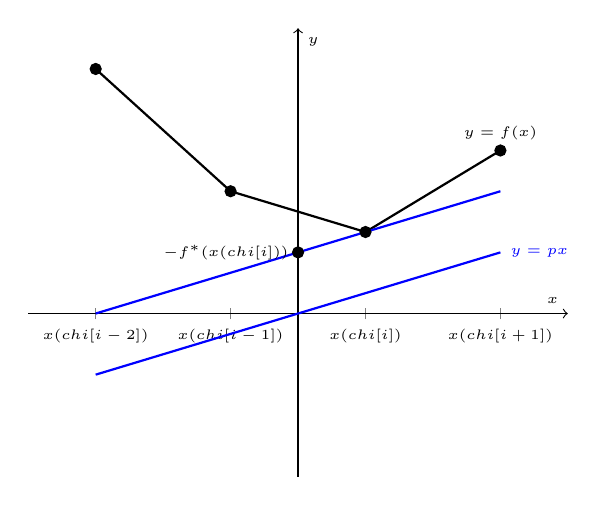
\begin{tikzpicture}
        \begin{axis}[
            xlabel={$x$},
            ylabel={$y$},
            ymin=-1, ymax=1.75,
            xmin=-2, xmax=2,
            xtick={-1.5,-0.5,0.5,1.5}, % x軸の目盛り
            xticklabels={$x(chi[i-2])$,$x(chi[i-1])$,$x(chi[i])$,$x(chi[i+1])$},
            ytick=\empty,
            axis lines=middle,
            axis line style={->},
            font=\tiny,
        ]

        % 直線の描画
        \addplot [black, thick, mark=none] coordinates {(-1.5,1.5) (-0.5,0.75)};
        \addplot [black, thick, mark=none] coordinates {(-0.5,0.75) (0.5,0.5)};
        \addplot [black, thick, mark=none] coordinates {(0.5,0.5) (1.5,1)} node[above, sloped] {$y=f(x)$};


        \addplot [blue, thick, mark=none] coordinates {(-1.5,0) (1.5,0.75)};
        \addplot [blue, thick, mark=none] coordinates {(-1.5,-0.375) (1.5,0.375)} node[right, sloped] {$y=px$};
        % 点の描画
        \addplot [only marks, mark=] coordinates {
        (-1.5,1.5)
        (-0.5,0.75)
        (0.5,0.5)
        (1.5,1)
        };
        \addplot [only marks, mark=] coordinates {(0,0.375)} node[left] {$-f^*(x(chi[i]))$};


        \end{axis}
    \end{tikzpicture}
    \caption{Legendre Fenchel変換の意味}
    \label{gra:legendre_mean}
\end{figure}




例として、$f(x) = \alpha |x|^2$とする。
このとき、
\begin{align*}
f^*(x) &= \displaystyle \sup_{p\in \Omega}{[x \cdot p - f(p)]} \quad (g(p) = x \cdot p - f(p))\\
           &=\displaystyle \sup_{p\in \Omega}{[x \cdot p - \alpha |p|^2]}\\
           &= \displaystyle \sup_{p\in \Omega}{[- \alpha(p^2 - \frac{1}{\alpha}xp)]}\\
           &= \displaystyle \sup_{p\in \Omega}{[- \alpha(p - \frac{1}{2 \alpha}x)^2 +  \frac{1}{4 \alpha}x^2]}\\
           &=  \frac{1}{4 \alpha}|x|^2 + \sup_{p\in \Omega}{[- \alpha(p - \frac{1}{2 \alpha}x)^2]}\\
           &= \frac{1}{4 \alpha}|x|^2 \qquad (\because  \text{$p = \frac{1}{2 \alpha}x$のとき,$g(p)$はsup.  $\Rightarrow f^*$は $p = \frac{1}{2 \alpha}x$のとき成立})\\
           &= \frac{1}{4 \alpha^2}f(x)\\
\end{align*}
よって、$\alpha = \frac{1}{2}$のとき、$f^*(x) = f(x)。$
また、$g(p)$が最大になるのは$p = \frac{1}{2 \alpha}x$のときである
$(g( \frac{1}{2 \alpha}x) = x \cdot \frac{1}{2 \alpha}x - \alpha  \frac{1}{4 \alpha^2}x^2 =  \frac{x^2}{4 \alpha} = f^*(x))$。
さらに、
$g(p) = x \cdot p - f(p)= x \cdot p - \alpha |p|^2$
であることから、
$g'(p) = 0 \Leftrightarrow x - 2 \alpha p = 0 \Leftrightarrow x - f'(p) = 0 \, (\because f'(x) = 2 \alpha x) \Leftrightarrow f'(p) = x$ 。

よって一般に、 $f(x) = \alpha |x| ^2$のとき、$f^*(p)$となる$x$は $f'(p) = x$より、ある点$p$での$f$の微分になり、 
かつ$x = f'(p) = 2\alpha p$ 。

つまり「$f^*(p)= sup_x\{p \cdot x - f(x) \} $の$x$を求めること」は 「$f'(p)$を求めること」に等しい。
よって Legendre-Fenchel transformとは,凸関数のある点$(x(chi[i]), y(chi[i])$における接線の傾き(微分)$p[j]$を求めるものである。


ここで$\alpha = \frac{1}{2}$のとき、 $f^*(x) = f(x) かつf'(p) = x = 2\alpha p = p$。

従って「$v[i]: (x(chi[i+1]), y(chi[i+1]))$と$(x(chi[i]), y(chi[i]))$を結んだ線分の傾き」$=$ 「$(x(chi[i]), y(chi[i]))$での接線の傾き(微分)」になる。
つまり、$\alpha = \frac{1}{2}$のとき、 $p$は$x$座標の分割であるので、十分小さい分割を取れば、 $p[j] = v[i]$となる$p$が必ず存在する.

特に凸関数ならば、$f^*(x)$は減少しない関数なので、$v[i]$も減少しない。
よって、$v[i] < p[j] \leq v[i+1]$となるものを見つけることができる(図\ref{gra:legendre})。この時、

\begin{center}
    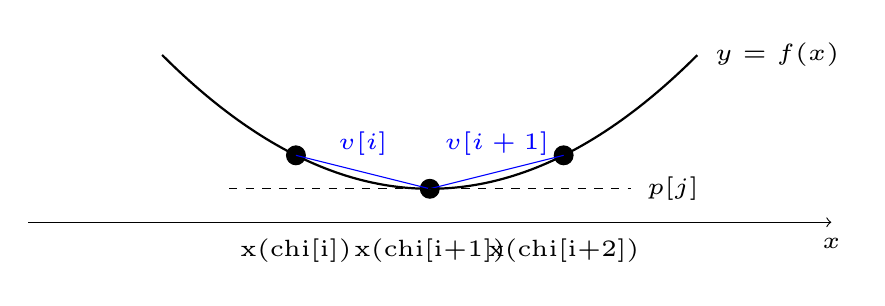
\begin{tikzpicture}[scale=1.7, transform shape]
        % グラフの描画
        \draw[->] (-3,0) -- (3,0) node[below, font=\tiny] {$x$};
        
        % 関数の描画
        \draw[black, thick, domain=-2:2, samples=100] plot (\x, {0.25*\x*\x + 0.25}) node[right, font=\tiny] {$y = f(x)$};
        
        % 点の描画
        \foreach \x/\y/\label in {-1/0.5/x(chi[i]), 0/0.25/x(chi[i+1]), 1/0.5/x(chi[i+2])}
            \filldraw (\x,\y) circle (2pt) node[below, font=\tiny] at (\x,0) {\label};
        
        % 直線の描画
        \draw[blue] (-1,0.5) -- (0,0.25) node[midway, above, font=\tiny] {$v[i]$};
        \draw[blue] (0,0.25) -- (1,0.5) node[midway, above, font=\tiny] {$v[i+1]$};
        
        % x=0での接線
        \draw[black, dashed] (-1.5,0.25) -- (1.5,0.25) node[right, sloped, font=\tiny] {$p[j]$};
        
    \end{tikzpicture}
    \captionof{figure}{Legendre Fenchel-1}
    \label{gra:legendre}
\end{center}


上記を踏まえ、Legendre-Fenchel変換のアルゴリズムAlgorithm\ref{al:legendre}に示す。

\begin{algorithm}[tb]
    \caption{Legendre-Fenchel Transform}
    \label{al:legendre}
    \begin{algorithmic}[1]
        \State \textbf{Input:} array $x, y = f(x)$ (coordinates of function $f$), $p$
        \State $chi, v \gets$ convex hull$(x, y) $
        \State $t \gets \{\}$
        \State iopt $\gets \{0,0, \dots, 0\} \quad \text{(ipot is same shape of array } x$) 
        \State $i \gets 0$
        \For {$j$, $p$ in enumerate($p$)}
            \While{$p > v(i)$}
                \State $i \gets i + 1$
            \EndWhile
            \State iopt($j$) = chi($i$)
            \State $t \gets t \cup x(\text{chi}($i$)) * p - y(\text{chi}($i$))$
        \EndFor
        \State \textbf{return} $t$, iopt
    \end{algorithmic}
\end{algorithm}

Legendre-Fenchel変換のアルゴリズムは以下のアイデアに基づいている:
\begin{enumerate}
    \item 関数$f \in \mathcal{C}$の凸包conv $f$を求める。(convex hull algorithm)
    \item 繰り返し
    \begin{enumerate}
        \item $(x(chi[i+1]), y(chi[i+1]))$と$(x(chi[i]), y(chi[i]))$を結んだ線分の傾き$v[i] \le p[j]$となる座標の添字番号$chi[i]$を見つける。
        \item $(x(chi[i]), y(chi[i]))$におけるLegendre-Fenchel変換を計算し、配列$t$に保存する。
    \end{enumerate}
\end{enumerate}
%%%%%%%%%%%%%%%%%%%%%%%%%%%%%%%%%%%%%%%%%%%%%%%%%%%%%%%%%%%%%%%%%%%%%%%%%%%%%%%%%%%%%%%%%%%%%%%%%%%%%%%%%%%%%%%%%%%%%%%%%%%%%%%%%%%%%%%%%%%

\subsection{Algorithm: $c$-変換}
\label{sect:al_c-tra}
$\varphi^c(p) = \frac{1}{\tau}\inf_x\left\{\frac{|x-p|^2}{2} - \tau\varphi(x)\right\}$について考える。
このときc変換は以下のようになる。
\begin{align*}
    \varphi^c(p) &= \frac{1}{\tau} \inf_x\left\{\frac{|x-p|^2}{2} - \tau \varphi(x)\right\}\\
              &= \frac{1}{\tau}  \left(\frac{|p|^2}{2} + \inf_x\left[- \left\{x \cdot p - \frac{|x|^2}{2} + \tau\varphi(x) \right\}\right]\right)\\
              &= \frac{1}{\tau}  \left(\frac{|p|^2}{2} - \sup_x\left[x \cdot p - \left\{\frac{|x|^2}{2} - \tau\varphi(x)\right\}\right]\right)\\
              &= \frac{1}{\tau}  \left(\frac{|p|^2}{2} - \sup_x\left\{x \cdot p - \psi(x)\right\} \qquad (\because \psi(x) = \frac{|x|^2}{2} - \tau\varphi(x))\right)\\
              &= \frac{1}{\tau}  \left(\frac{|p|^2}{2} - \psi^*(p)\right)\\
    \\
    \varphi^{cc}(q) 
              &= \frac{1}{\tau} \inf_p\left\{\frac{|p-q|^2}{2} - \tau \varphi^c(p)\right\}\\
              &= \frac{1}{\tau}\left(\frac{|q|^2}{2} + \inf_p\left[- \left\{p \cdot q - \frac{|p|^2}{2} + \tau\varphi^c(p) \right\}\right]\right)\\
              &= \frac{1}{\tau}\left(\frac{|q|^2}{2} - \sup_p\left[p \cdot q - \left\{\frac{|p|^2}{2} - \tau\varphi^c(p)\right\}\right]\right)\\
              &= \frac{1}{\tau}\left(\frac{|q|^2}{2} - \sup_p\left[p \cdot q - \left\{\frac{|p|^2}{2} - \left(\frac{|p|^2}{2} - \psi^*(p)\right)\right\}\right]\right)\\
              &= \frac{1}{\tau}\left(\frac{|q|^2}{2} - \sup_p\left[p \cdot q - \psi^*(p)\right]\right) \\
              &= \frac{1}{\tau}\left(\frac{|q|^2}{2} - \varphi^{**}(q)\right)
\end{align*}

上記を踏まえ、$c$-変換のアルゴリズムをAlgorithm\ref{al:c-transform}に示す。
アルゴリズムでは、$c$-変換を$\inf_x\left\{\frac{|x-p|^2}{2} - \varphi(x)\right\}$としている。
そのため、アルゴリズム中の$\varphi(x)$を$\tau\varphi(x)$、returnされた値$\frac{1}{2} p^2 - t$を$\frac{1}{\tau}\left(\frac{1}{2} p^2 - t\right)$とすることによって、実際の$c$-変換の値を計算している。

\begin{algorithm}[tb]
    \caption{c-transform}
    \label{al:c-transform}
    \begin{algorithmic}[1]
        \State \textbf{Input:} array $x,y = \varphi(x)$ (coordinates of function $f$), $p(=x)$
        \State $\psi(x) \gets \frac{1}{2} x^2 - \varphi(x)$
        \State $t$, index $\gets$ Legendre-Fenchel transform$(x, \psi, p)$
        \State \textbf{return} $\frac{1}{2} p^2 - t, $ index
    \end{algorithmic}
\end{algorithm}


\subsection{Algorithm: 最適輸送写像(押し出し測度)}
\label{sect:al_pushforward}
$\varphi, \psi$がどちらも$c$-凹のとき、押し出し測度$T_{\varphi \#} \mu$および$T_{\psi \#} \delta U^*(- \psi^c)$は、
\begin{equation*}
    T_{\phi \#} \mu (y) =\mu(y - \tau \nabla \phi(y))|\det (I - \tau D^2 \varphi(y))|
\end{equation*}
\begin{equation*}
    T_{\psi \#} \delta U^* (- \psi^c)(x) =\delta U^* (- \psi^c)(x - \tau \nabla \psi(x))|\det (I - \tau D^2 \psi(x))|
\end{equation*}
である。

押し出し測度のアルゴリズムは以下のアイデアに基づいている。
    
\begin{enumerate}
    \item 入力パラメータ:
    \begin{itemize}
        \item \texttt{mu}: セルごとの初期密度を表す配列。
        \item \texttt{phi\_c}: セルごとの位相関数を表す配列。
        \item \texttt{h}: グリッド間のセルサイズ。
    \end{itemize}

    \item 初期化:
    \begin{itemize}
        \item \texttt{t\_mu}: 結果を格納するための配列を、\texttt{mu} と同じ形状で初期化。
    \end{itemize}

    \item 各セルに対して以下を繰り返す:
    \begin{enumerate}
        \item セル番号iの近傍の3つのセル(um,u,up)における$\varphi$の$c$-変換を求める。
        \item $\varphi$の$c$-変換に対するセル$i$における勾配(dphi\_c)を中心差分法で計算する。
        \item セル \texttt{i} におけるヘッセ行列の行列式 det ($\text{det}(I - D^2\phi_c)$) を計算する。
        \item 変形前の座標系における位置xcellの計算する。
        \item xcellに最も近いセルのインデックスtiとその次のセルtioを計算する。
        \item tiとtioにおける密度を線形補間して、xcellでの密度 mu\_inter を計算する。
        \item セルiにおける押し出し測度t\_mu[i]($T_{\varphi \#} \mu$, $T_{\psi \#} \delta U^*(- \psi^c)$)を計算する。
    \end{enumerate}

\end{enumerate}

上記を踏まえ、押し出し測度のアルゴリズムをAlgorithm \ref{alg:push_forward}に示す。
\begin{algorithm}
    \caption{Push Forward}
    \label{alg:push_forward}
    \begin{algorithmic}[1]
        \State \textbf{Input:}{$\mu, \varphi_c, h$}
        \State Initialize $t_\mu$ as a zero array of the same shape as $\mu$
        \State $n \gets \text{shape}(\varphi_c)[0]$
        \State Initialize empty lists $l_{\nabla\varphi_c}$ and $l_{\text{det}}$
        
        \For{$i$ in range($n$)}
            \State $um \gets \varphi_c[\max(i-1, 0)]$
            \State $u \gets \varphi_c[i]$
            \State $up \gets \varphi_c[\min(i+1, n-1)]$
            
            \State $\nabla\varphi_c \gets \frac{up - um}{2h}$
            \State $l_{\nabla\varphi_c}.\text{append}(\nabla\varphi_c)$
            
            \State $\text{det} \gets 1 - \frac{up - 2u + um}{h^2}$
            \State $l_{\text{det}}.\text{append}(\text{det})$
            
            \State $x_{\text{cell}} \gets i - \frac{\nabla\varphi_c}{h}$
            \State $ti \gets \text{int}(\min(\max(\lfloor x_{\text{cell}} \rfloor, 0), n - 1))$
            \State $tio \gets \min(ti + 1, n - 1)$
            
            \State $\mu_{\text{inter}} \gets \mu[ti] \left(1 - (x_{\text{cell}} - \lfloor x_{\text{cell}} \rfloor)\right) + \mu[tio] \left(x_{\text{cell}} - \lfloor x_{\text{cell}} \rfloor\right)$
            
            \State $t_\mu[i] \gets \mu_{\text{inter}} \cdot \text{det}$
        \EndFor
        
        \State \textbf{return} $t_\mu$
    \end{algorithmic}
\end{algorithm}


\section{The back-and-forth methodを用いたJKOスキームの実装}
\label{sect:algorithm}
本論文ではThe back-and-forth methodを使用して、多孔質勾配方程式
\[
    \rho_t = \frac{{\partial \rho}}{{\partial t}} = \gamma\Delta (\rho^m), \quad (\rho \geq 0, m > 1)
\]
を解く。
ただし、
\[
    \rho(t, x) := \overline{\rho}(\gamma(t+t_0), x) 
\]
とする。このとき
$
    \partial_t\rho = \gamma\partial_t\overline{\rho} 
$
より、
\begin{equation}
    \left\{ \,
    \begin{aligned}
        \rho_t - \gamma\Delta(\rho^m) & = 0 \\
        \rho(0, x) & = \overline{\rho}(\gamma t_0, x)
    \end{aligned}
    \right.
\end{equation}
と考えることができる。
初期データは
\[
    \rho(0,x) = M\delta_0(x)
\]
で与えられるとする。
ここで、\(\gamma > 0\)は拡散の速度を制御する定数、\(M > 0\)は初期総質量、\(\delta_0\)は原点を中心とする標準的なディラックのデルタ分布とする。
\(m > 1\)の場合、この方程式はエネルギー
\[
    U(\rho) = \int_\Omega \frac{\gamma}{m - 1}\rho(x)^m dx 
\]
のWasserstein勾配流となる。
領域\(R\)上で閉じた解が存在し、これはBarenblatt solutionとして知られている。
Barenblatt solutionは安定性条件を必要としないため、非常に有効な近似解を得ることができる。
Barenblatt solutionは以下のように与えられる(ただし、$(\cdot)_+ = max(\cdot, 0), \alpha = \frac{1}{m + 1}, \beta = \frac{1}{m + 1}$):
\begin{equation}
    \label{eq:barenblatt}
    \rho(t,x)= \frac{1}{t^\alpha}\left(b - \frac{m - 1}{2m}\frac{\beta |x|^2}{t^{2\beta}} \right)_+^{\frac{1}{m - 1}}
\end{equation}

ここで例として$m = 2$のとき、
\begin{equation}
    \label{eq:barenblatt:m=2}
    \rho(t,x)= \frac{1}{t^{\frac{1}{3}}}\left(b - \frac{1}{12} \frac{ |x|^2}{t^{\frac{2}{3}}} \right)_+
\end{equation}
となる。さらに、
\begin{align*}
    \rho(t, x) = 0 &\iff \frac{1}{t^{\frac{1}{3}}}\left(b - \frac{1}{12} \frac{ |x|^2}{t^{\frac{2}{3}}} \right) = 0,\\
                    &\iff b = \frac{1}{12}\frac{|x|^2}{t^{\frac{2}{3}}}, \\
                    &\iff |x|^2 = 12t^{\frac{2}{3}}b \iff x = \pm \sqrt{12t^{\frac{2}{3}}b},
\end{align*}



\begin{align*}
    \int^{+\infty}_{-\infty} \rho(t, x)dx &= 2 \int^{\sqrt{12t^{\frac{2}{3}}b}}_0 \frac{1}{t^{\frac{1}{3}}}\left(b - \frac{1}{12} \frac{|x|^2}{t^{\frac{2}{3}}}\right)dx,\\
                                            &= \frac{2}{t^{\frac{1}{3}}}\left(b r - \frac{r^3}{3 \cdot 12 t^{\frac{2}{3}}}\right) \qquad \left(\because r := \sqrt{12t^{\frac{2}{3}}b}\right),\\
                                            &= \frac{2}{t^{\frac{1}{3}}}\left(b r - \frac{12t^{\frac{2}{3}}b r}{3 \cdot 12 t^{\frac{2}{3}}}\right) = \frac{2}{t^{\frac{1}{3}}}\frac{2}{3}br,\\
                                            &= \frac{2}{t^{\frac{1}{3}}}\frac{2}{3}b \cdot 2\cdot \sqrt{3} t^{\frac{1}{3}},\\
                                            &= \frac{8}{\sqrt{3}}b^{\frac{3}{2}} =: M  \qquad \Longrightarrow b = \left(\frac{\sqrt{3}}{8} M \right)^{\frac{2}{3}}.
\end{align*}



したがって、質量が正方形の境界に達するまでの時間$t_c$まで、$\Omega = [- \frac{1}{2}, \frac{1}{2}]$の上の解と一致することがわかる。
初期条件のディラックのデルタ関数は扱いにくいため、高さ$h_0 > 0$を固定し、時間$t_0 > 0$から開始することにする。
ここで$t_0$は、$\|\rho(0, \cdot)\|_{L^\infty}= \|\overline{\rho} (\gamma t_0, \cdot)\|_{L^\infty} = h_0$となるように選ぶ。
ただし、$t_0$は以下のように求めることができる。
\begin{align*}
    \|\rho(0, \cdot)\|_{L^\infty} = \|\overline{\rho} (\gamma t_0, \cdot)\|_{L^\infty} &= \overline{\rho}(\gamma t_0, 0) = \frac{1}{(\gamma t_{0})^{\frac{1}{3}}} b\ = h_0\\
    \Longrightarrow \, t_0 = \frac{1}{\gamma}\left(\frac{b}{h_0}\right)^3
\end{align*}
さらに、Barenblatt solutionは時間$t_c$までの間にのみ有効であるため、時間$t \in [t_0, 2.0+t_0]$のみを考慮する。
このBarenblatt solutionを基準として使用して、各アルゴリズムの精度と効率をテストしていく。
解の精度は$L^1$ノルムを使用して以下のように誤差を求めることができる。
\begin{equation}
    \label{eq:error}
    \text{error} = \frac{1}{N_\tau} \sum_{n = 0}^{N_\tau} \int_\Omega |\overline{\rho}(\gamma(n \tau + t_0), x) - \overline{\rho}^{(n)}(x)|\, dx
\end{equation}
ここでnは離散的な時間ステップを示し、$\tau$は時間のステップサイズを表す。
ただし、$N_\tau = \lfloor \frac{2}{\tau} \rfloor$であり、$\overline{\rho}(n\tau + t_0, x)$はBarenblatt solutionであり、
$\overline{\rho}^{(n)}$は初期データ$\overline{\rho}^{(0)}(x) = \overline{\rho}(\gamma t_0, x) = $から始まる$n$回目のJKOスキームである。
また$\varphi^{(n+1)}$を求める際、the back-and-forth methodを使用する。
ただし$\|\delta U^*(- \varphi) - T_{\varphi \#} \mu \|_{L^1(\Omega)}$が$\varepsilon (\text{実験では}\varepsilon = 10^{-3}, 10^{-5}, 10^{-6}\text{を使用})$未満、
もしくは繰り返しが100回より多くなるまでthe back-and-forth methodを繰り返す。

アルゴリズム実装のため、各関数の値を確認しておく。
エネルギー関数は
\[
    U(\rho) := \frac{\gamma}{{m-1}} \int \rho^m \, dx, \quad \delta U(\rho) = \frac{m \gamma}{m-1} \rho^{m-1}
\]
であり、$U$のLegendre Fenchel変換$U^*$は
\[
     U^*(- \varphi) = \sup_{\rho \in P} \int \left(- \frac{\gamma}{m-1}\rho^m - \rho\varphi\right) \, dx
\]
であった。このときLemma. \ref{lem:rho_opt}より、$U^*(- \varphi)$を最大化させる$\rho_*$は
\begin{equation}
    \label{eq:m=2rho}
    \rho_*(x) = \delta U^*(- \varphi) =  \left( \frac{m-1}{m\gamma}(C - \varphi)_+ \right)^{\frac{1}{m-1}} 
\end{equation}

となる。
以上を用いて、多孔質勾配方程式$(m=2)$におけるthe back-and-forth methodの離散化したアルゴリズムをAlgorithm \ref{al:baf}に示す。

\begin{algorithm}
    \caption{Discretised the back-and-forth method}
    \label{al:baf}
    \begin{algorithmic}[1]
        \State \textbf{Input:} $\mu = \rho^{(0)} = \max\left(\frac{1}{(\gamma t_0)^{1/3}}\left(b - \frac{1}{12}\frac{x^2}{(\gamma t_0)^{2/3}}\right),0\right), \varphi_0 = \delta U(\rho^{(0)}) = \frac{m \gamma}{m-1} \left(\rho^{(0)}\right)^{m-1}$
        \While{$\text{diff} \geq \varepsilon$}
            \If{$\text{count} > 100$}
                \State \textbf{break}
            \EndIf
            \State $\rho \leftarrow \left(\frac{m-1}{m\gamma}\max(c - \varphi, 0)\right)^{1/(m-1)}$
            \State $\varphi, \psi, \text{pfwd} \leftarrow \text{ascent}(\varphi, \psi, \mu, \rho)$ (Algorithm \ref{al:ascent})
            \State $\text{diff} \leftarrow \sum \left|\rho - \text{pfwd}\right| \cdot h$
    
            \State $\psi_c, \_ \leftarrow \text{c\_transform}(x, \tau \cdot \psi, x)$ 
            \State $\psi_c \leftarrow \frac{\psi_c}{\tau}$
    
            \State $\rho \leftarrow \left(\frac{m-1}{m\gamma}\max(c - \psi_c, 0)\right)^{1/(m-1)}$
            \State $\psi, \varphi, \text{pfwd} \leftarrow \text{ascent}(\psi, \varphi, \rho, \mu)$
    
            \State $\text{count} \leftarrow \text{count} + 1$
        \EndWhile
    \end{algorithmic}
\end{algorithm}
ここで、Algorithm \ref{al:baf}の7行目ascentとはAlgorithm \ref{al:ascent}を指す。
また、Algorithm \ref{al:ascent}の8行目gauss$(\rho - \text{pfwd}, \Theta_1, \Theta_2)$ とは、
\[
    (\Theta_1 \text{Id} - \Theta_2 \Delta)u = f
\]
において、$f = \rho - \text{pfwd}$のとき$u = \text{lp}$を求めるものである。
    \begin{algorithm}
        \caption{Ascent in Algorithm \ref{al:baf}}
        \label{al:ascent}
        \begin{algorithmic}[1]
            \State \textbf{Input:} $\varphi$, $\varphi_c$, $\mu$, $\rho$
            \State $\varphi_c, \_ \leftarrow \text{c\_transform}(x, \tau \cdot \varphi, x)$ 
            \State $\varphi_c \leftarrow \frac{\varphi_c}{\tau}$
        
            \State $n\mu \leftarrow \max(\lVert\mu\rVert_\infty)$
            \State $\Theta_1 \leftarrow \frac{1}{2\gamma}$
            \State $\Theta_2 \leftarrow \tau \cdot n\mu$
        
            \State $\text{pfwd} \leftarrow \text{push\_forward}(\mu, \tau \cdot \varphi, h)$ 
            \State $lp \leftarrow \text{gauss}(\rho - \text{pfwd}, \Theta_1, \Theta_2)$ 
            \State $\varphi \leftarrow \varphi + lp$ 
            
            \State $\varphi_c, \_ \leftarrow \text{c\_transform}(x, \tau \cdot \varphi, x)$
            \State $\varphi_c \leftarrow \frac{\phi_c}{\tau}$
    
            \State \textbf{return}  $\varphi, \varphi_c, \text{pfwd}$ 
        \end{algorithmic}
    \end{algorithm}
\chapter{最適輸送写像のアルゴリズム}
\label{ch:optmap_algorithm}
\section{最適輸送写像}
\label{sect:最適輸送写像}

$I$および$J$の勾配(\ref{eq:J-gradient})(\ref{eq:I-gradient})を計算するには、押し出し測度も計算する必要がある。
密度$\mu$および可逆な写像$T: \Omega \to \Omega$が与えられた場合、ヤコビアンの公式を使用して押し出し測度 $T_\# \mu$を計算できる。

The back-and-forth methodの構造のおかげで、$\varphi, \psi$がどちらも$c$-凹の場合にのみ、$T_{\varphi \#} \mu$および$T_{\psi \#} \delta U^*(- \psi^c)$を計算すればよい。
Proposition. \ref{prop:transport map}より、
\[
    T_\varphi ^{-1}(y) = y - \tau \nabla \varphi(y), T_\psi^{-1}(x) = x - \tau \nabla \psi(x),
\]
\[
    y = T_\phi(x), \quad x = T^{-1}_\phi (y), \quad dx = |\det \nabla T^{-1}_\phi (y)| dy 
\]

$I$および$J$の勾配(\ref{eq:J-gradient})(\ref{eq:I-gradient})、さらに$J$と$I$ の一次変分(\ref{eq:delta J}), (\ref{eq:delta I})から、
$T_{\varphi \#} \mu$, $T_{\psi \#} \delta U^*(- \psi^c)$は以下のように求められる。
\begin{align*}
    T_{\phi \#} \mu (A) &= \int_A T_{\phi \#} \mu (x)\, dx = \mu(T^{-1}_\phi (A))\\
                        &= \int_{T^{-1}_\phi (A)} \mu(x) \, dx\\
                        &= \int_A \mu \left( T^{-1}_\phi(y) \right) |\det \nabla T^{-1}_\phi (y)|\, dy = \int_A \frac{\mu \left( T^{-1}_\phi(y) \right)}{|\det \nabla T\left(T^{-1}_\phi (y)\right)|}\, dy\\
                        &= \int_A \mu(y - \tau \nabla \phi(y))|\det (I - \tau D^2 \phi(y))|\, dy\\
                        &= \mu(y - \tau \nabla \phi(y))|\det (I - \tau D^2 \phi(y))|
\end{align*}
\begin{align*}
    T_{\psi \#} \delta U^* (- \psi^c) (A)   &= \int_A T_{\psi \#} \delta U^* (- \psi^c) (y)\, dy =  \delta U^* (- \psi^c)(T^{-1}_\psi (A))\\
                                            &= \int_{T^{-1}_\psi (A)} \delta U^* (- \psi^c) (y) \, dx\\
                                            &= \int_A  \delta U^* (- \psi^c)  \left(T^{-1}_\psi (x) \right) |\det \nabla T^{-1}_\psi (x)|\, dy = \int_A \frac{\ \delta U^* (- \psi^c)  \left( T^{-1}_\psi(x) \right)}{|\det \nabla T\left(T^{-1}_\psi (x)\right)|}\, dy\\
                                            &= \int_A \delta U^* (- \psi^c)(x - \tau \nabla \psi(x))|\det (I - \tau D^2 \psi(x))|\, dx\\
                                            &= \delta U^* (- \psi^c)(x - \tau \nabla \psi(x))|\det (I - \tau D^2 \psi(x))|
\end{align*}

\begin{equation}
    \label{eq:pushforward Tphi}
    T_{\phi \#} \mu (y) =\mu(y - \tau \nabla \phi(y))|\det (I - \tau D^2 \phi(y))|
\end{equation}
\begin{equation}
    \label{eq:pushforward Tpsi}
    T_{\psi \#} \delta U^* (- \psi^c)(x) =\delta U^* (- \psi^c)(x - \tau \nabla \psi(x))|\det (I - \tau D^2 \psi(x))|
\end{equation}
%実装する際、私たちのアルゴリズムではこれらの量をシンプルな中心差分スキームを使用して計算します。

\section{最適輸送写像のアルゴリズム}
\chapter{実験および結果} 
\label{ch:実験及び結果}
\section{}

\section{まとめ}
\chapter{おわりに} \label{ch:conclusion}
本論文の目的であった偏微分方程式の解法の一つであり特に非線形偏微分方程式の数値解法として有用なthe back-and-forth methodを用いて非線形である多孔質勾配方程式の解を求め、他の解法との比較を行うことができた。
back-and-forth methodは他の解放と比べて大きい時間ステップサイズであっても誤差を少なく近似することができた。
これは$\rho$を直接求めるのではなく、$\rho_*(x) = \delta U^*(- \varphi)$で$\rho$を再現するため、
不連続な$\rho$の台の境界でショックが起凝らないことと双対問題を解くことで制約がない状態で計算できるからである。

ただし、グリッドサイズに合わせ、適切な時間ステップ$\tau$とback-and-forth methodの反復を抜ける条件の$\|\delta U^*(- \varphi) - T_{\varphi \#} \mu \|_{L^1(\Omega)} < \varepsilon$を適切に取る必要がある。

今後の展望としては多孔質勾配方程式の$m$の値を大きくすること、2・3次元などで考えることなどが挙げられる。

\appendix
\chapter{ふろく}
\section{緒言}
\bibliographystyle{plain}
\bibliography{ref}  % BibTeXファイルの指定

% \chapter*{研究業績}
\addcontentsline{toc}{chapter}{研究業績}
\section*{本研究に関係するもの}
%	\subsection*{投稿論文}
%		\begin{enumerate}
%			\renewcommand{\labelenumi}{[\arabic{enumi}]}
%		\end{enumerate}
	
	\subsection*{国際会議論文}
%		\begin{enumerate}
%			\renewcommand{\labelenumi}{[\arabic{enumi}]}
%		\end{enumerate}
	
	\subsection*{国内発表}
%		\begin{enumerate}
%			\renewcommand{\labelenumi}{[\arabic{enumi}]}
%		\end{enumerate}
		
\section*{その他の業績}
	\subsection*{投稿論文}
%		\begin{enumerate}
%			\renewcommand{\labelenumi}{[\arabic{enumi}]}
%		\end{enumerate}
%		
	\subsection*{国際会議論文}
%		\begin{enumerate}
%			\renewcommand{\labelenumi}{[\arabic{enumi}]}
%		\end{enumerate}
		
	\subsection*{国内発表}
%		\begin{enumerate}
%			\renewcommand{\labelenumi}{[\arabic{enumi}]}
%		\end{enumerate}
\section*{受賞}
%	\begin{enumerate}
%		\renewcommand{\labelenumi}{[\arabic{enumi}]}
%	\end{enumerate}\Delta 
\chapter*{謝辞}
\addcontentsline{toc}{chapter}{謝辞}
感謝・・・・っ!圧倒的感謝っ・・・・!
\end{document}
